\addappheadtotoc
\appendix

%\customlink{Definitions_derivations_and_tricks}
\chapter{Definitions, derivations and tricks}
\label{app:definitions}

Paleomagnetism is famous for its use of a large number of incomprehensible acronyms.  Here we have them gathered together along with definitions and the Section numbers where they are explained in more detail.  You  will find here  a table of physical constants and paleomagnetic parameters used in the text as well as a table listing common statistics used in paleomagnetism.   After the tables, there are a few sections with useful mathematical tricks.  



\section{Definitions}

\begin{center}
\begin{longtable}{ll}
\caption[Acronyms]{ Acronyms in paleomagnetism. }
\label{tab:acronyms}\\

\hline
Acronym & Definition: Section \#  \\
\hline
\endfirsthead

%
\multicolumn{2}{l}{\it  -- continued from previous page} \\
\hline
Acronym &  Definition: Section \#  \\
\hline
\endhead

\hline \multicolumn{2}{r}{{\it Continued on next page --}} \\
\endfoot
\hline
\endlastfoot

AMS& Anisotropy of magnetic susceptibility: Section~\ref{sect:chimeas}\\
APWP&Apparent polar wander path: Section~\ref{sect:apwp}\\
AF&Alternating field demagnetization:  Section~\ref{sect:demag}\\
ARM & Anhysteretic remanent magnetization: Section~\ref{sect:arm}\\
ChRM& Characteristic remanent magnetization: Section~\ref{sect:chrm}\\
CNS&Cretaceous Normal Superchron: Section~\ref{sect:gpts}\\
CRM& Chemical remanent magnetization: Section~\ref{sect:crm}\\
DGRF&Definitive geomagnetic reference field: Section~\ref{sect:igrf}\\
DRM& Detrital remanent magnetization:  Section~\ref{sect:drm}\\
E/I& Elongation/inclination correction method: Section~\ref{sect:tk03}\\
FC& Field cooled: Section~\ref{sect:delta}\\
GAD& Geocentric axial dipole: Section~\ref{sect:gad}\\
GHA&Greenwich hour angle: Appendix~\ref{app:sundec}\\
GPTS&Geomagnetic polarity time scale: Chapter 15\\
GRM & Gyroremanent magnetization: Section~\ref{sect:arm}\\
IGRF&International geomagnetic reference field: Section~\ref{sect:igrf}\\
IZZI& Infield-zero field/ zero field-infield paleointensity protocol: Section~\ref{sect:KTT}\\
IRM& Isothermal remanent magnetization: Sections~\ref{sect:uniaxial} and s\ref{sect:irm}\\
MD&Multi-domain:  Chapter 4\\
MDF&Median destructive field: Section~\ref{sect:crittemp}\\
MDT&Median destructive temperature: Section~\ref{sect:crittemp}\\
NRM & Natural remanent magnetization: Chapter 7\\
pARM& Partial anhysteretic remanence:  Section~\ref{sect:arm}\\
pDRM&Post-depositional detrital remanent magnetization: Section~\ref{sect:drm}\\
PSD&Pseudo-single domain: Chapter 4\\
PSV&Paleosecular variation of the geomagnetic field: Section~\ref{sect:historical}\\
pTRM& Partial thermal remanence:   Section~\ref{sect:trm}\\
sIRM& Saturation IRM: See $M_r$\\
SD&Single domain:  Chapter 4\\
SP&Superparamagnetic:  Section~\ref{sect:tau}\\
SV&Secular variation:  Section~\ref{sect:historical}\\
TRM& Thermal remanent magnetization: Section~\ref{sect:trm}\\
VADM& Virtual axial dipole moment:  Section~\ref{sect:vdm}\\
VDM& Virtual dipole moment:  Section~\ref{sect:vdm}; Equation~\ref{eq:vdm}\\
VDS& Vector difference sum: Section~\ref{sect:vds}\\
VGP&Virtual geomagnetic pole: Section~\ref{sect:vgp}\\
VRM & Viscous remanent magnetization: Section~\ref{sect:vrm}\\
SQUID&Superconducting quantum interference device: Section~\ref{sect:meas}\\
UT&Universal time (Greenwich mean time): Appendix~\ref{app:sundec}\\
ZFC& Zero-field cooled: Section~\ref{sect:delta}\\
\hline
\end{longtable}
\end{center}


\begin{center}
\begin{longtable}{ll}
\caption[ Physical Parameters and Constants]{ Physical Parameters and Constants. }
\label{tab:physconstants}\\
\hline
Symbol & Definition: Section \#  \\
\hline
\endfirsthead

%
\multicolumn{2}{l}{\it  -- continued from previous page} \\
\hline
Symbol &  Definition: Section \#  \\
\hline
\endhead

\hline \multicolumn{2}{r}{{\it Continued on next page --}} \\
\endfoot
\hline
\endlastfoot

$\chi$ & Magnetic susceptibility:   The slope relating induced \\
 &  \hskip 1em magnetization to an applied field: Section~\ref{sect:mag}\\
 $\chi_{ARM}$& ARM susceptibility: Section~\ref{sect:trends}\\
$\chi_b$& Bulk magnetic susceptibility: Section~\ref{sect:mag}; Equation~\ref{eq:chi}\\
$\chi_d$& Diamagnetic susceptibility: Section~\ref{sect:dia}\\
$\chi_f$& Ferromagnetic susceptibility: Section~\ref{sect:ferro}\\
$\chi_{fd}$& Frequency dependent: Section~\ref{sect:chifd}\\
$\chi_h$ & High-frequency susceptibilty:  Section~\ref{sect:rosenbaum} \\
$\chi_{hf}$ & High-field susceptibilty: Section~\ref{sect:chi}\\
$\chi_{i}$ & Initial susceptibilty: Section~\ref{sect:chi} \\
$\chi_l$ & Low-frequency susceptibilty: Section~\ref{sect:rosenbaum} \\
$\chi_p$& Paramagnetic susceptibility: Section~\ref{sect:para}\\
$\delta_{FC}$& Verwey transition temperature jump while \\
&cooling in a field: Section~\ref{sect:delta}\\
$\delta_{ZFC}$& Verwey transition temperature jump while\\
& cooling in zero field: Section~\ref{sect:delta}\\
$\Delta M$ curve&Curve defined by subtracting the ascending\\
& \hskip 1em from the descending curves in a\\
&\hskip 1em hysteresis loop: Section~\ref{sect:uniaxial}\\
$\lambda,\phi$& Latitude, Longitude\\
$\mu_o$&Permeability of free space: 
(4$\pi$ x 10$^{-7}$ Hm$^{-1}$): Section~\ref{sect:BvH}\\
$\tau$& Relaxation time: Section~\ref{sect:tau}; Equation~\ref{eq:tau}\\
$\theta_m$&Magnetic co-latitude: Section~\ref{sect:eqarea}; Equation~\ref{eq:mcolat}\\
$\theta$&Co-latitude: Section~\ref{sect:potential}\\
$a_{ij}$&Direction cosines: Appendix~\ref{app:dircosines} \\
$[a_m]$ & Magnetic activity: Section~\ref{sect:drmint}\\
$a$& The radius of the Earth (6.371 x 10$^6$ m): Section~\ref{sect:igrf}\\
$\B$&Magnetic induction: Section~\ref{sect:flux}\\
$C$&Frequency factor (10$^{10}$ s$^{-1}$): Section~\ref{sect:tau}\\
$D$&Declination: Section~\ref{sect:comp}; Equation~\ref{eq:DI}\\
$E$&Elongation: Table~\ref{tab:params}\\
$I$&Inclination: Section~\ref{sect:comp}; Equation~\ref{eq:DI}\\
$g_m^l, h_m^l$& Gauss coefficients: Section~\ref{sect:igrf}\\
$\H$&Magnetic field: Section~\ref{sect:H}\\
$H_{cr}$& Coercivity of remanence; field required to reduce
saturation\\
&\hskip 1em IRM to zero: Section~\ref{sect:flipping}\\
$H_c$&Coercivity; the magnetic field required to change the magnetic\\
&\hskip 1em moment of a particle from one easy axis to another: Section~\ref{sect:flipping}\\
$I$&Inclination: Section~\ref{sect:comp}; Equation~\ref{eq:DI}\\
$k$&Boltzmann's constant (1.381 x 10$^{-23}$ JK$^{-1}$): Section~\ref{sect:para}\\
$K_i$ & AMS measurement: Appendix~\ref{app:K15}\\
$K_u$&Constant of uniaxial anisotropy energy: Sections~\ref{sect:K1} and ~\ref{sect:shape}\\
$\m$&Magnetic moment: Section~\ref{sect:moment}\\
$\m_b$&Bohr magneton (9.27 x 10$^{-24}$ Am$^2$):  Section~\ref{sect:atomic}\\
$\M$&Magnetization:  Section~\ref{sect:mag}\\
$M_{eq}$& Equilibrium magnetization:    Section~\ref{sect:vrm}\\
$M_r$& Saturation remanence (also sIRM): Section~\ref{sect:uniaxial}\\
$M_s$ & Saturation magnetization;   the magnetization measured in the
\\
 & \hskip 1em  presence of a saturating field: Section~\ref{sect:uniaxial}\\
$P_l^m$&Schmidt polynomials: Section~\ref{sect:igrf}\\
$\s$& Six elements of $ \chi_{ij}$; $s_1=\chi_{11}, s_2=\chi_{22},
s_3=\chi_{33}, s_4=\chi_{12},s_5=\chi_{23}, s_6=\chi_{13}$:\\
& Section~\ref{sect:chimeas}; Equation~\ref{eq:kj}\\
$R_x$&IRM cross-over value:  Section~\ref{sect:interactions}\\
$T$&Absolute temperature (in kelvin)\\
$T_b$&Blocking temperature:  Section~\ref{sect:trm}\\
$T_c$&Curie (N\'eel) temperature:  Section~\ref{sect:ferro},~\ref{sect:crittemp}\\
$T_h$&Hopkinson Effect: Section~\ref{sect:crittemp}\\
$T_m$&Morin transition: Section~\ref{sect:crittemp}\\
$T_o$&Absolute zero: Section~\ref{sect:ferro}\\
$T_p$& Pyrrhotite transition: Section~\ref{sect:crittemp}\\
$T_v$&Verwey temperature:  Section~\ref{sect:K1},~\ref{sect:crittemp}\\
$v$&Volume\\
$v_b$&Blocking volume:  Section~\ref{sect:crm}\\
\hline
\end{longtable}
\end{center}


\begin{center}
\begin{longtable}{ll}
\caption[ Statistics]{ Common statistics in paleomagnetism. }
\label{tab:statistics}\\

\hline
Statistic & Definition: Section \#  \\
\hline
\endfirsthead

%
\multicolumn{2}{l}{\thetable{}\it  -- continued from previous page} \\
\hline
Statistic &  Definition: Section \#  \\
\hline
\endhead

\hline \multicolumn{2}{r}{{\it Continued on next page --}} \\
\endfoot
\hline
\endlastfoot

$\alpha_{95}$& Radius of circle (cone) of 95\% confidence (Fisher): Section~\ref{sect:fisher}, Equation~\ref{eq:a95}\\
$\delta$& Residual errors for AMS measurements: Section~\ref{sect:chimeas}, Equation~\ref{eq:kdel}\\
$\epsilon_{ij}$&Semi-angles of Hext uncertainty ellipses: Section~\ref{sect:chimeas}, Equation~\ref{eq:eij}\\
$\kappa$& Fisher precision parameter:  Section~\ref{sect:fisher},Equation~\ref{eq:fishdis}\\
$\eta_{95}, \zeta_{95}$& Semi-angles of directional 95\%  uncertainty
 ellipses:\\
& Section~\ref{app:kent}, Equation~\ref{eq:zeta}\\
${\bm \tau, \V}$& Eigenvalues and eigenvectors of tensors: Section~\ref{app:eigen}, Equation~\ref{eq:eig} \\
$k$& Estimate of $\kappa$:  Section~\ref{sect:fisher}, Equation~\ref{eq:k}\\
CSD&Circular standard deviation (Fisher): Section~\ref{sect:fisher}, Equation~\ref{eq:csd}\\
$dm$&Uncertainty in the meridian (longitude)\\
& of a paleomagnetic pole: Section~\ref{sect:fisher}, Equation~\ref{eq:dpdm}\\
$dp$&Uncertainty in the parallel (latitude)\\
& of a paleomagnetic pole: Section~\ref{sect:fisher}, Equation~\ref{eq:dpdm}\\
$F,F_{12}, F_{23}$& Significance tests for anisotropy (Hext): Section~\ref{sect:hextE}, Equation~\ref{eq:fij}\\
MAD&Maximum angular deviation of principal eigenvector (Kirschvink):\\
& Section~\ref{sect:BFL}, Equation~\ref{eq:mad}\\
MAD$_{plane}$&MAD of the pole to a best-fit plane (Kirschvink):\\
&  Section~\ref{sect:BFL}, Equation~\ref{eq:madP}\\
$M_u, M_e$& Significance tests for uniform and exponential
distributions: Section~\ref{sect:fishtests}  \\
& Appendix~\ref{app:qq}, Equations~\ref{eq:Mu}, and ~\ref{eq:Me}\\
$N$& Number of samples, specimens or sites\\
$n_f$& Number of degrees of freedom: Section~\ref{sect:hext}, Equation~\ref{eq:So}  \\
$R$&Resultant vector length of unit vectors,  Section~\ref{sect:fisher}, Equation~\ref{eq:R}\\
$R_o$&Critical value of $R$ for non-random distribution 
(Watson):\\
& Section~\ref{sect:Ro}, Equation~\ref{eq:Ro}\\
$S_f$ & Scatter of VGPs - corrected for within site scatter: Equation~\ref{eq:Sf}\\
$S_p$ & Scatter of VGPs: Equation~\ref{eq:Sp}\\
$S_o$& Residual sum of squares of errors (Hext): Section~\ref{sect:hext}, Equation~\ref{eq:So} \\
$T$& Orientation tensor: Appendix~\ref{app:eigen}, Equation~\ref{eq:tmatrix}\\
\hline
\end{longtable}
\end{center}

\section{Derivations}
\subsection{Langevin function for a paramagnetic substance}
\label{app:langevin}

Here we derive the Langevin function for a paramagnetic substance with magnetic moments $M$m$m$ in an applied field $H$ at temperature $T$.  If we make  the assumption that there is no preferred alignment
within the substance, we can assume that the number of moments ($n(\alpha)$) between
angles $\alpha$ and $\alpha + d\alpha$ with respect to $\H$ is
proportional to the  solid angle $\sin\alpha d\alpha$ and the probability density
function, \ie

\beq
n(\alpha) d\alpha \propto \exp \bigl({ -E_m\over {kT}} \bigr) \sin \alpha d\alpha,
\label{eq:nalpha}
\eeq

\noindent where $E_m$ is the magnetic energy. 
When  we measure the induced magnetization, we really measure only the 
component of the moment 
parallel to the applied field, or $n(\alpha) m \cos
\alpha$.  The net induced magnetization $M_I$ of a population of particles
with volume $v$ is therefore:

\beq
{M_I = }{m\over v}  \int_0^{\pi} n(\alpha)\cos \alpha d \alpha.
\label{eq:MI}
\eeq

\noindent By definition,  $n(\alpha)$ integrates to $N$,  the total
number of moments, or
\beq
{N=} {\int_0^{\pi} n(\alpha)d\alpha } .
\label{eq:N}
\eeq

The total saturation moment of a given population of $N$ individual 
magnetic moments $m$ is $Nm$.
The saturation value of magnetization $M_s$ is thus $Nm$ normalized by 
the volume $v$. Therefore, the magnetization expressed as the fraction of
saturation is:

$$
{M\over {M_s}} =  { {\int_0^{\pi} n(\alpha ) \cos \alpha d\alpha}\over
{\int_0^{\pi} n(\alpha )d\alpha }}
$$
$$
\hskip 12pt =  { {\int_o^{\pi} e^{(m\mu_o H \cos \alpha )/kT}\cos 
\alpha \sin \alpha
d\alpha}\over { \int_o^{\pi} e^{(m\mu_o H\cos
\alpha )/kT}\sin \alpha
d\alpha}}.
$$

\noindent
By substituting $a=m\mu_oH/kT$ and $\cos \alpha =x$, we write


\beq
{
M\over {M_s}
} =
{N 
  { 
 {\int_{-1}^{1} e^{a x}xdx}
 \over
  {\int_{-1}^1 e^{a x}dx}
  }
}
  = \bigl( 
{
 {
 {e^{a} + e^{-a}}
 \over
 {e^{a} - e^{-a}}
 }
 - {1\over{a} }
}
\bigr),
\eeq
and finally
\beq
{M\over {M_s}} =
{ [\hbox{coth }a -
{
1\over{a}
}]=\mathcal{L} (a).
}
\label{eq:Langapp} 
\eeq


\subsection{Superparamagnetism}
\label{app:superparamagnetism}

The derivation of superparamagnetism follows closely that of paramagnetism 
whereby the probability of finding a magnetization vector an angle $\alpha$ away from the direction of the applied field is give by:

\begin{equation}
n(\alpha )d\alpha = 2\pi n_o e^{({{M_sBv\cos \alpha}\over {kT}})}\sin \alpha
d\alpha .
\label{eq:ccnalpha}
\end{equation}

\noindent
The total magnetization contributed by the $N$ moments is:

\begin{equation}
{M\over {M_s}} = \int_0^{\pi} \cos \alpha n(\alpha )d\alpha.
\label{eq:ccMint}
\end{equation}
\noindent
Combining  Equations\ref{eq:ccnalpha}) and ~\ref{eq:ccMint} we
get:
$$
{M\over {M_s}} = N { {\int_0^{\pi} n(\alpha ) \cos \alpha d\alpha}\over
{\int_0^{\pi} n(\alpha )d\alpha }}
$$

$$
\hskip 12pt = N { {\int_o^{\pi} e^{(M_sBv\cos \alpha )/kT}\cos \alpha \sin \alpha
d\alpha}\over { \int_o^{\pi} e^{(M_sBv\cos
\alpha )/kT}\sin \alpha
d\alpha}}.
$$
\noindent
By substituting $a= M_sBv/kT$ and $\cos \alpha =x$,  and remembering Equation~\ref{eq:Langapp},    we can write:

\begin{equation}
{
M\over {M_s}
} =
{N 
  { 
 {\int_1^{-1} e^{a x}xdx}
 \over
  {\int_1^{-1} e^{a x}dx}
  }
}
  = N\mathcal{L} (a).
\end{equation}

\noindent
So  finally
\begin{equation}
{M\over {M_s}} =
{ N\mathcal{L} (a).
}
\end{equation}




\section{Useful tricks}

In this section, we have assembled assorted mathematical and plotting techniques that come in handy through out this book. 


%\customlink{Spherical_trigonometry}
\subsection{Spherical trigonometry}
 \label{app:strig}
 
 Spherical trigonometry has widespread applications throughout the book.  It is used in the transformations of observed directions to virtual poles (Chapter 2) and transformation of coordinate sytems, to name a few.   Here we summarize the two most useful relationships:  the 
 \index{Law of!sines}
 {\it Law of Sines} and the 
 \index{Law of!cosines}
 {\it Law of Cosines}.     
 
\begin{figure}[h!tb]
%\epsfxsize 8cm
%\centering \epsffile{EPSfiles/strig.eps}
\centering  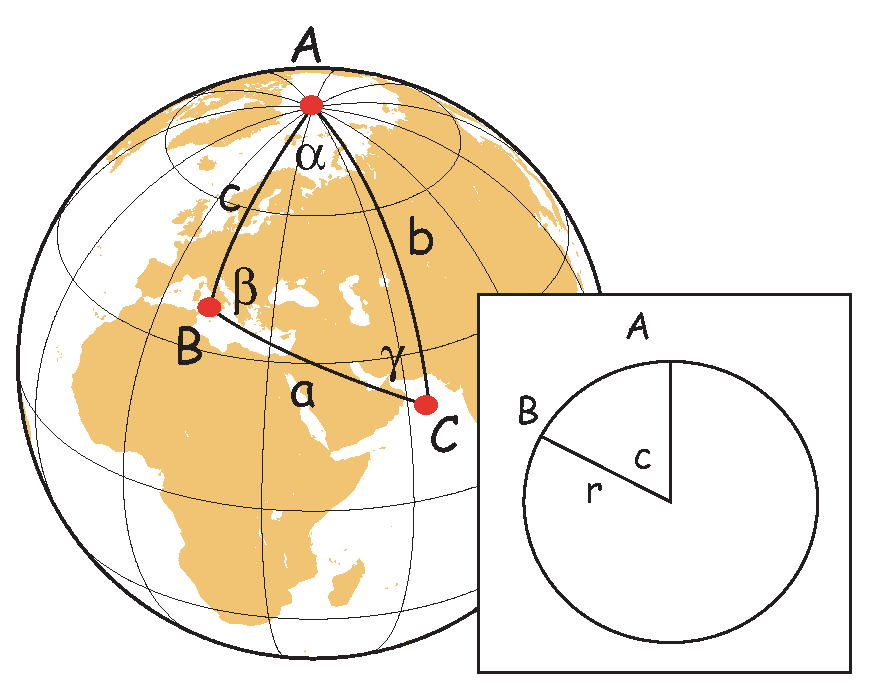
\includegraphics[width=8 cm]{EPSfiles/strig.eps}
\caption{Rules of spherical trigonometry.  $a,b,c$ are all great circle tracks
on a sphere which form a triangle with apices $A,B,C$. 
The lengths of $a,b,c$ on  a unit sphere  are equal to
 the angles subtended by
radii that intersect the globe at the apices,
as shown in the inset. $\alpha,\beta,\gamma$ are the angles
between the great circles. }
\label{fig:strig} 
\end{figure}


In Figure~\ref{fig:strig},  $\alpha, \beta$ and $\gamma$ are  the angles
between the great circles labelled $a$, $b$, and $c$. On a unit sphere, 
$a,b$ and $c$ are also the angles
subtended by radii that intersect the globe at the apices A, B, and C (see inset on
Figure~\ref{fig:strig}).  
Two formulae from spherical trigonometry come in handy in paleomagnetism, the Law of Sines:

\beq {\sin \alpha \over \sin a}={\sin \beta \over \sin b}={\sin \gamma \over \sin c},
\label{eq:lawsin}
\eeq
 \noindent and the Law of Cosines:
 
\beq \cos a = \cos b \cos c + \sin b \sin c \cos \alpha.
\label{eq:lawcos}
 \eeq



\subsection{Vector addition}
\label{app:vectors}

\begin{figure}[htb]
%\centering \epsffile{EPSfiles/vectors.eps}
\centering  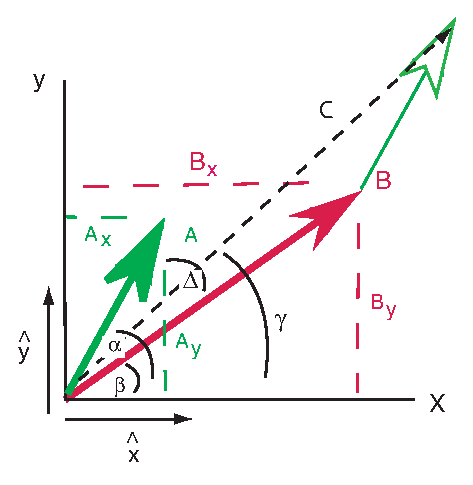
\includegraphics{EPSfiles/vectors.eps}
\caption{Vectors $\A$ and $\B$, their components A$_{x,y}$, B$_{x,y}$ and the angles between
them and the $X$ axis, $\alpha$ and $\beta$.  The angle between the two vectors is $\alpha$
-$\beta$ = $\Delta$.  Unit vectors in the directions of the axes are $\hat x$ and $\hat y$ respectively.   }
\label{fig:vectors}
\end{figure}



To add the two vectors (see Figure~\ref{fig:vectors}) $\A$ and $\B$,  we break each
vector into components $A_{x,y}$ and $B_{x,y}$.  For example, $A_x=|A|\cos{\alpha},
A_y=|A|\sin{\alpha}$ where $|A|$ is the length of the vector $\A$.  The
components of the resultant vector $\C$ are: $C_x = A_x +B_x, C_y=A_y+B_y$.   These
can be converted back to polar coordinates of magnitude and angles if desired, whereby:

$$
|C| = \sqrt {C_x^2+C_y^2} \hbox{and} \gamma= \cos^{-1} { {C_x}\over{ {|C|}}}.
$$ 

\subsection{Vector subtraction}

To subtract two vectors, compute the components as in addition, but the components of the
vector difference
$\C$ are:  $C_x = A_x -B_x, C_y=A_y-B_y$.  

%\customlink{Vector_multiplication}
\subsection{Vector multiplication}
\label{app:vecmult}

There are two ways to multiply vectors.  The first is the dot product whereby $\A \cdot
\B= A_xB_x + A_yB_y$.  This is a scalar and is actually the cosine of the angle between
the two vectors if the $\A$ and $\B$ are taken as unit vectors (assume a magnitude of
unity in the component calculation.    
 
 \begin{figure}[h!tb]
%\epsfxsize 6cm
%\centering \epsffile{EPSfiles/cross.eps}
\centering  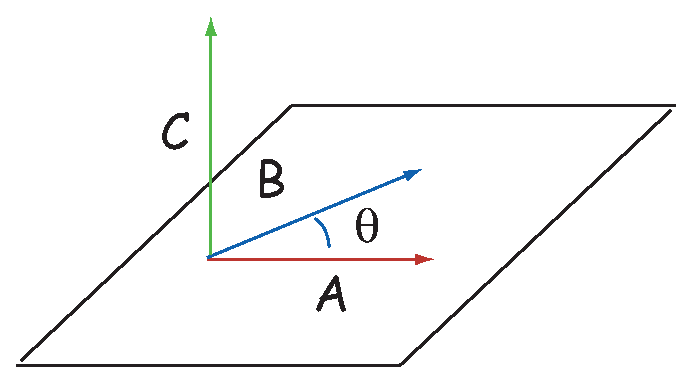
\includegraphics[width=6 cm]{EPSfiles/cross.eps}
\caption{Illustration of cross product of vectors $A$ and $B$ separated by angle $\theta$ to get the orthogonal vector $C$.  }
\label{fig:cross}
\end{figure}

 
 
 The other way to perform vector multiplication is the cross
product (see Figure~\ref{fig:cross}), which  produces a vector orthogonal to both $\A$ and $\B$  and whose components are given by:

$$
C = \det \left|\, \matrix{
\hat x & \hat y &\hat z \cr
A_x & A_y & A_z\cr
B_x & B_y & B_z\cr}\right|.
$$

To calculate the determinant, we follow these rules:

$$
C_x=A_yB_z - A_zB_y,
C_y=A_zB_x - A_xB_z,
C_z=A_xB_y - A_yB_x.
$$

or

$$C_i = A_jB_k-A_kB_j \hskip .25in i\neq j \neq k.
$$
 

\subsection{Tricks with tensors}
\label{app:tensors}

\index{anisotropy!tensors}%
Vectors belong to a more general concept called tensors.  While a vector describes a magnitude of something in a given direction, tensors allow calculation of magnitudes as a function of orientation.  Velocity is a vector relating speed to direction, but speed may change depending on direction, so we might need a tensor to calculate speed as a function of direction.   Many properties in Earth science require tensors, like the indicatrix in mineralogy which relates the speed of light to crystallographic direction, or the relationship between stress and strain.  Tensors in paleomagnetism are used, for example,  to transform coordinate systems and to characterize the anisotropy of  magnetic properties such as susceptibility.    We will cover transformation of coordinate systems in the following.  

 
 \subsubsection{Direction cosines}
 \label{app:dircosines}
 
We use direction cosines in paleomagnetism  in a variety of applications, from mineralogy to transformation from specimen to geographic or stratigraphic coordinate systems.  Direction cosines are the cosines of the angles between different axes in  given coordinate systems, here $X$ and $X'$ respectively  (see, e.g., Figure~\ref{fig:transform}a.)   The direction cosine $a_{12}$  is the cosine of the angle between the $X_1$ and the $X'_2$, $\alpha_{12}$ axes.    We can define four of these direction cosines to fully describe the relationship between the two coordinate systems:

$$
\matrix{
a_{11} = \cos \alpha_{11}, a_{21} = \cos \alpha_{21},\cr
a_{12} = \cos \alpha_{12}, a_{22} = \cos \alpha_{22}.\cr
}
$$

\noindent The first subscript always refers to the $X$ system and the second refers to the $X'$.  

\begin{figure}[h!tb]
%\epsfxsize 10cm
%\centering \epsffile{EPSfiles/dircosines.eps}
\centering  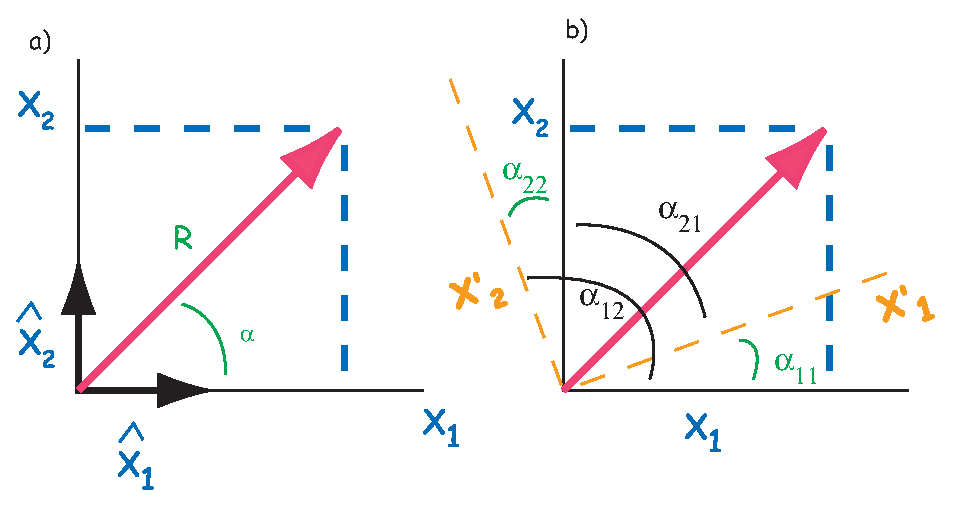
\includegraphics[width=10 cm]{EPSfiles/dircosines.eps}
\caption{Definition of direction cosines in two dimensions.  a) Definition of vector in one set of coordinates, $x_1, x_2$.  b) Definition of angles relating $X$ axes to $X'$.  }
\label{fig:transform}
\end{figure}

%\customlink{Changing_coordinate_systems}
\subsubsection{Changing coordinate systems}
\label{app:coord}
\index{coordinate systems!transformation}% 

One application of using direction cosines is the transformation of coordinates  systems from one set ($X$) to a new set $X'$.  
To find new coordinates $x'_1, x'_2,..$ from the old ($x_1, x_2,...$), we have:

$$
\matrix{
x_1' = a_{11} x_1 + a_{12} x_2,\cr
x_2' = a_{21} x_2 + a_{22} x_2.}
$$

In three dimensions we have:  

$$
\matrix{
x_1' = a_{11} x_1 + a_{12} x_2 + a_{13} x_3,\cr
x_2' = a_{21} x_1 + a_{22} x_2 + a_{23} x_3,\cr
x_3' = a_{31} x_1+ a_{32} x_2 + a_{33} x_3,}
$$

\noindent which can also be written as:

\beq
{\pmatrix{x'_1\cr x'_2\cr x'_3\cr}} = 
{\pmatrix{
 a_{11}&a_{12}&a_{13}\cr
 a_{21}&a_{22}&a_{23}\cr
 a_{31}&a_{32}&a_{33}\cr
}}
{\pmatrix{x_1\cr x_2\cr x_3\cr}},
\label{eq:matrot}
\eeq


\noindent with a short cut notation as:  $x'_i = a_{ij} x_j$.  However we write this, it  means that for each axis $i$, just sum through the $j$'s for all the dimensions.   The matrix $a_{ij}$ is an example of a 3 x 3 tensor and equations of the form $A_i = B_{ij} C_j$ relating two vectors with a tensor will be used throughout the book.  A more common notation is with bold-faced variables which indicate vectors or tensors, e.g., ${\bf A} = {\bf B} \cdot {\bf C}$.  

\begin{figure}[htb]
%\epsfxsize 12cm
%\centering \epsffile{EPSfiles/transform.eps}
\centering  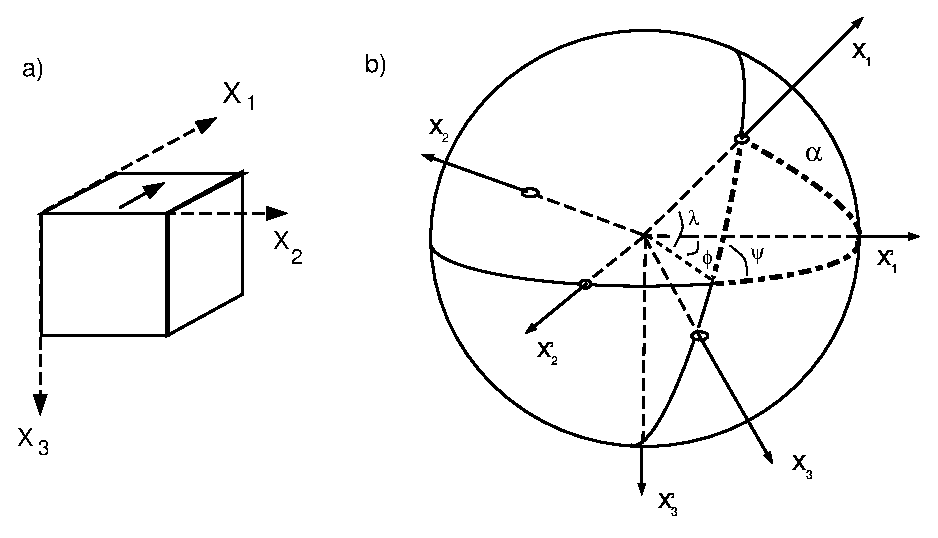
\includegraphics[width=12 cm]{EPSfiles/transform.eps}
\caption {
a) Sample coordinate system.
b) Trigonometric relations between two cartesian coordinate systems, $\X_i$ and
$\X'_i$.  $\lambda,\phi,\psi$ are all known and the angles between the various axes
can be calculated using spherical trigonometry.  
For example, the angle $\alpha$
 between $\X_1$ and $\X_1'$ forms one side of the
triangle shown by dash-dot lines.  Thus,
$\cos \alpha = \cos \lambda \cos \phi + \sin \lambda \sin \phi \cos \psi
$. 
[Figure from Tauxe, 1998.]}
\label{fig:trans}
\end{figure}

Now we would like to apply this to changing coordinate systems for a paleomagnetic specimen in the most general case.  
 The specimen 
coordinate system is  
defined by a right-hand rule where the thumb ($\X_1$) is  
directed  parallel
to an arrow marked on the sample, the index finger ($\X_2$) is in the same
plane but at right angles and clockwise to $\X_1$ and the middle finger ($\X_3$) is
perpendicular to the other two (Figure~\ref{fig:trans}a). 
The transformation of coordinates ($x_i$) from the $\X_i$ 
axes to the coordinates in the desired $\X'$ coordinate system
requires the determination of the direction cosines as described in Appendix~\ref{app:dircosines}.  The various $a_{ij}$ can be calculated using
\index{spherical!trigonometry}%
spherical trigonometry as in Appendix~\ref{app:strig}.    For example, $a_{11}$ for the
general case depicted in Figure~\ref{fig:trans} is $\cos \alpha$, which is given by the
\index{Law of!cosines}
Law of Cosines  (see Appendix~\ref{app:strig}) by using appropriate values, or:

$$
\cos \alpha = \cos \lambda \cos \phi +
\sin \lambda \sin \phi \cos \psi.
$$

The other $a_{ij}$ can be calculated in a similar manner.  In the case of most
coordinate system rotations used in paleomagnetism, 
$X_2$ is in the same plane as $X'_1$ and
$X'_2$ (and is horizontal) so $\psi$ = 90$^{\circ}$. This  problem is much simpler.
The directions cosines for the case where $\psi = 90^{\circ}$ are:

\begin{equation}
a=\pmatrix{
\cos \lambda \cos \phi & - \sin \phi & - \sin \lambda \cos \phi\cr
\cos \lambda \sin \phi & \cos \phi & - \sin \lambda \sin \phi \cr
\sin \lambda & 0& \cos \lambda \cr} .
\label{eq:aij}
\end{equation}

The new coordinates can be obtained from Equation~\ref{eq:matrot}, as follows:

\beq
\matrix{
x'_1 = a_{11}x_1 + a_{12}x_2 + a_{13}x_3\cr
x'_2 = a_{21}x_1 + a_{22}x_2 + a_{23}x_3\cr
x'_3 = a_{31}x_1 + a_{32}x_2 + a_{33}x_3.\cr}
\label{eq:newx}
\eeq

\noindent
The declination and inclination can be calculated by inserting these values
in  the equations in Chapter 2.   

%\customlink{polerot} % Lori don't change this
\subsubsection{Method for rotating points on a globe using finite rotation poles}
\label{app:polerot}

  Given  the coordinates of the point on the globe $P_p$ with latitude $\lambda_p$, longitude $\phi_p$  the  finite rotation pole $P_f$ with latitude $\lambda_f$,   longitude $\phi_f$, the way to transform coordinates is as follows (you should also review Appendix~\ref{app:coord}).  

\begin{enumerate}

\item Convert the latitudes and longitudes to cartesian coordinates by:
$$ 
P_1=\cos\phi \cos \lambda, P_2 = \sin \phi \cos \lambda, P_3 = \sin \lambda
$$
\noindent where $P$ is the point of interest.  

\item  Set up the rotation matrix $R$ as:

$$
\matrix{
R_{11} = P_{f1}P_{f1}(1-\cos \Omega) + \cos \Omega \cr
R_{12} = P_{f1}P_{f2}(1-\cos \Omega) -  P_{f3} \sin \Omega \cr
R_{13} = P_{f1}P_{f3}(1-\cos \Omega) + P_{f2}\sin \Omega \cr
R_{21} = P_{f2}P_{f1}(1-\cos \Omega) + P_{f3}\sin  \Omega \cr
R_{22} = P_{f2}P_{f2}(1-\cos \Omega) + \cos \Omega \cr
R_{23} = P_{f2}P_{f3}(1-\cos \Omega) -P_{f1}\sin  \Omega \cr
R_{31} = P_{f3}P_{f1}(1-\cos \Omega) - P_{f2} \sin  \Omega \cr
R_{32} = P_{f3}P_{f2}(1-\cos \Omega) + P_{f1}\sin  \Omega \cr
R_{33} = P_{f3}P_{f3}(1-\cos \Omega) + \cos \Omega \cr}.
$$


\item The coordinates of the transformed pole ($P_t$) are:
$$
\matrix{
P_{t1} = R_{11} P_{p1} + R_{12}P_{p2}+R_{13}P_{p3}\cr
P_{t2} = R_{21} P_{p1} + R_{22}P_{p2}+R_{23}P_{p3}\cr
P_{t3} = R_{31} P_{p1} + R_{32}P_{p2}+R_{33}P_{p3}\cr
},
$$
\noindent which can be converted back into latitude and longitude in the usual way (see Chapter 2).  
\end{enumerate}

\begin{center}
\begin{longtable}{|l|lll|lll|lll|lll|}
\caption[Finite Rotations for Gondwanda continents ]{Finite rotations for selected Gondwana continents.  Rotates continent to South African fixed coordinates. AUS: Australia, ANT: East Antarctica; IND: India; SAM: South American Craton. [Rotations of Torsvik et al. (2008) - see for additional data.] }
\label{tab:gondrot}\\

\hline
 Age &  & AUS &  &  & ANT &  &  & IND &  &  & SAM\\
\hline
Ma & $\lambda$ & $\phi$ & $\Omega$ & $\lambda$ & $\phi$ & $\Omega$ & $\lambda$ & $\phi$ & $\Omega$ & $\lambda$ & $\phi$ & $\Omega$  \\
\hline
% %\\

\endfirsthead
\multicolumn{8}{l}%
{\tablename\ \thetable{}\it  -- continued from previous page} \\
\hline
Ma & $\lambda$ & $\phi$ & $\Omega$ & $\lambda$ & $\phi$ & $\Omega$ & $\lambda$ & $\phi$ & $\Omega$  & $\lambda$ & $\phi$ & $\Omega$ \\
% \\
\hline
\endhead

\hline \multicolumn{8}{r}{{\it Continued on next page --}} \\
\endfoot
%\hline \multicolumn{8}{c}{Rotations from  Torsvik et al. 2008.}\\
%% %\\
\hline
\endlastfoot

5 & 9.7 & 54.3 & -3.3 & 8.2 & -49.4 & 0.8 & 22.7 & 32.9 & -2.3 & 62.1 & -40.2 & 1.6\\
10 & 10.4 & 52.8 & -6.2 & 8.2 & -49.4 & 1.5 & 23.8 & 33.1 & -4.6 & 61.8 & -40.3 & 3.3\\
15 & 11.5 & 49.8 & -9 & 9.8 & -48.4 & 2.1 & 27.1 & 27.4 & -6 & 59.6 & -38.1 & 5.4\\
20 & 12.4 & 48 & -11.8 & 10.7 & -47.9 & 2.8 & 29.6 & 23.9 & -7.5 & 58.5 & -37.1 & 7.5\\
25 & 12.9 & 48.3 & -15 & 11.4 & -48.2 & 3.8 & 25.1 & 33.2 & -10.3 & 57.7 & -36.4 & 9.6\\
30 & 12.8 & 49.9 & -18.1 & 11.8 & -48.3 & 4.8 & 22.5 & 38.5 & -13.3 & 56.7 & -34.5 & 11.9\\
35 & 13.5 & 50.8 & -20.9 & 12.5 & -46.1 & 6 & 22.6 & 41.3 & -15.9 & 56.5 & -33.4 & 14.3\\
40 & 14.1 & 52.7 & -22.1 & 13.6 & -41.5 & 7.4 & 25.5 & 42.7 & -17.4 & 57.1 & -32.6 & 16.6\\
45 & 14.4 & 54.7 & -22.9 & 11.1 & -41.1 & 8.5 & 24.2 & 40.1 & -19.7 & 57 & -31.4 & 18.6\\
50 & 14.7 & 56.5 & -23.6 & 9.1 & -40.9 & 9.6 & 24 & 34.2 & -23.5 & 58.2 & -31.2 & 20.5\\
55 & 14 & 57.3 & -24.7 & 9.4 & -43.5 & 10.3 & 22.1 & 29.2 & -28.3 & 60.7 & -31.9 & 22\\
60 & 12.9 & 57.9 & -25.7 & 10.6 & -47.4 & 10.8 & 19.5 & 25.2 & -34.4 & 62.5 & -32.8 & 23.3\\
65 & 13.6 & 58.8 & -26.3 & 8.1 & -47.7 & 11.3 & 19 & 21.9 & -40.2 & 63.7 & -33.5 & 24.6\\
70 & 17.3 & 60.2 & -26.3 & 0.4 & -43.3 & 12.2 & 20.5 & 18.9 & -44.4 & 63.5 & -33.4 & 26.1\\
75 & 19.8 & 63.3 & -26.7 & 3.7 & 138.9 & -13.8 & 21.8 & 18.2 & -47.3 & 63.2 & -33.9 & 28.6\\
80 & 20.5 & 68.5 & -26.6 & 2.7 & 142.7 & -16.1 & 22.3 & 18.2 & -49.1 & 62.7 & -34.3 & 31.5\\
85 & 19.8 & 74.6 & -26.9 & 0.6 & 144.7 & -18.8 & 21.8 & 22.1 & -53.8 & 61.2 & -34.3 & 34.4\\
90 & 17.7 & 80.9 & -28.9 & 1.4 & -37 & 22.3 & 20 & 27.5 & -58.8 & 59.1 & -34.5 & 37.3\\
95 & 15.9 & 86.2 & -31.1 & 2.9 & -38.3 & 25.8 & 20.7 & 28.1 & -57.8 & 57.2 & -34.7 & 40.3\\
100 & 18.4 & 89.3 & -30.7 & 3.1 & 146.5 & -26.8 & 21.3 & 28.8 & -56.8 & 55.7 & -34.8 & 43.3\\
105 & 17.9 & 95.6 & -32.6 & 5.5 & 148.9 & -30.3 & 21.9 & 29.6 & -55.9 & 54.3 & -34.9 & 46.4\\
110 & 17.3 & 101 & -34.8 & 7.4 & 150.7 & -33.9 & 22.6 & 30.3 & -54.9 & 53.1 & -35 & 49.5\\
115 & 16.8 & 105.6 & -37.4 & 9 & 152.3 & -37.6 & 23.3 & 31.1 & -54 & 52.2 & -35 & 51.7\\
120 & 16.4 & 109.4 & -40.3 & 10.3 & 153.6 & -41.3 & 24 & 32 & -53.1 & 51.6 & -35 & 52.8\\
125 & 15.7 & 110.3 & -42.3 & 9.4 & 152.4 & -43 & 23.4 & 34.8 & -55.2 & 50.7 & -33.9 & 54\\
130 & 15.9 & 111.6 & -44.4 & 9.1 & 151.5 & -45.3 & 21.2 & 36.2 & -60.1 & 50.1 & -32.8 & 54.9\\
135 & 15.9 & 113.1 & -46.6 & 8.6 & 150.9 & -47.6 & 21.2 & 36.2 & -61.6 & 50 & -32.5 & 55.1\\
140 & 15.6 & 113.7 & -48.3 & 8 & 150.1 & -49.2 & 21.9 & 37.5 & -61.5 & 50 & -32.5 & 55.1\\
145 & 15 & 113.1 & -50.5 & 7.3 & 148.1 & -50.7 & 22.6 & 39 & -62.5 & 50 & -32.5 & 55.1\\
150 & 15.5 & 113.5 & -52.5 & 7.4 & 147.1 & -52.6 & 24.1 & 40.4 & -62.9 & 50 & -32.5 & 55.1\\
155 & 17.6 & 115.7 & -54.3 & 9 & 148 & -55.4 & 26.9 & 41.2 & -61.6 & 50 & -32.5 & 55.1\\
160 & 19.5 & 117.8 & -56.2 & 10.5 & 148.8 & -58.2 & 29.8 & 42.1 & -60.5 & 50 & -32.5 & 55.1\\
165 & 19.5 & 117.8 & -56.2 & 10.5 & 148.8 & -58.2 & 29.8 & 42.1 & -60.5 & 50 & -32.5 & 55.1\\
170 & 19.5 & 117.8 & -56.2 & 10.5 & 148.8 & -58.2 & 29.8 & 42.1 & -60.5 & 50 & -32.5 & 55.1\\
175 & 19.5 & 117.8 & -56.2 & 10.5 & 148.8 & -58.2 & 29.8 & 42.1 & -60.5 & 50 & -32.5 & 55.1\\
180 & 19.5 & 117.8 & -56.2 & 10.5 & 148.8 & -58.2 & 29.8 & 42.1 & -60.5 & 50 & -32.5 & 55.1\\
185 & 19.5 & 117.8 & -56.2 & 10.5 & 148.8 & -58.2 & 29.8 & 42.1 & -60.5 & 50 & -32.5 & 55.1\\
190 & 19.5 & 117.8 & -56.2 & 10.5 & 148.8 & -58.2 & 29.8 & 42.1 & -60.5 & 50 & -32.5 & 55.1\\
195 & 19.5 & 117.8 & -56.2 & 10.5 & 148.8 & -58.2 & 29.8 & 42.1 & -60.5 & 50 & -32.5 & 55.1\\
200 & 19.5 & 117.8 & -56.2 & 10.5 & 148.8 & -58.2 & 29.8 & 42.1 & -60.5 & 50 & -32.5 & 55.1\\
205 & 19.5 & 117.8 & -56.2 & 10.5 & 148.8 & -58.2 & 29.8 & 42.1 & -60.5 & 50 & -32.5 & 55.1\\
210 & 19.5 & 117.8 & -56.2 & 10.5 & 148.8 & -58.2 & 29.8 & 42.1 & -60.5 & 50 & -32.5 & 55.1\\
215 & 19.5 & 117.8 & -56.2 & 10.5 & 148.8 & -58.2 & 29.8 & 42.1 & -60.5 & 50 & -32.5 & 55.1\\
220 & 19.5 & 117.8 & -56.2 & 10.5 & 148.8 & -58.2 & 29.8 & 42.1 & -60.5 & 50 & -32.5 & 55.1\\
225 & 19.5 & 117.8 & -56.2 & 10.5 & 148.8 & -58.2 & 29.8 & 42.1 & -60.5 & 50 & -32.5 & 55.1\\
230 & 19.5 & 117.8 & -56.2 & 10.5 & 148.8 & -58.2 & 29.8 & 42.1 & -60.5 & 50 & -32.5 & 55.1\\
235 & 19.5 & 117.8 & -56.2 & 10.5 & 148.8 & -58.2 & 29.8 & 42.1 & -60.5 & 50 & -32.5 & 55.1\\
240 & 19.5 & 117.8 & -56.2 & 10.5 & 148.8 & -58.2 & 29.8 & 42.1 & -60.5 & 50 & -32.5 & 55.1\\
245 & 19.5 & 117.8 & -56.2 & 10.5 & 148.8 & -58.2 & 29.8 & 42.1 & -60.5 & 50 & -32.5 & 55.1\\
250 & 19.5 & 117.8 & -56.2 & 10.5 & 148.8 & -58.2 & 29.8 & 42.1 & -60.5 & 50 & -32.5 & 55.1\\
255 & 19.5 & 117.8 & -56.2 & 10.5 & 148.8 & -58.2 & 29.8 & 42.1 & -60.5 & 50 & -32.5 & 55.1\\
260 & 19.5 & 117.8 & -56.2 & 10.5 & 148.8 & -58.2 & 29.8 & 42.1 & -60.5 & 50 & -32.5 & 55.1\\
265 & 19.5 & 117.8 & -56.2 & 10.5 & 148.8 & -58.2 & 29.8 & 42.1 & -60.5 & 50 & -32.5 & 55.1\\
270 & 19.5 & 117.8 & -56.2 & 10.5 & 148.8 & -58.2 & 29.8 & 42.1 & -60.5 & 50 & -32.5 & 55.1\\
275 & 19.5 & 117.8 & -56.2 & 10.5 & 148.8 & -58.2 & 29.8 & 42.1 & -60.5 & 50 & -32.5 & 55.1\\
280 & 19.5 & 117.8 & -56.2 & 10.4 & 148.8 & -58.2 & 29.8 & 42.1 & -60.5 & 50 & -32.5 & 55.1\\
285 & 19.5 & 117.8 & -56.2 & 10.5 & 148.8 & -58.2 & 29.8 & 42.1 & -60.5 & 50 & -32.5 & 55.1\\
290 & 19.5 & 117.8 & -56.2 & 10.5 & 148.8 & -58.2 & 29.8 & 42.1 & -60.5 & 50 & -32.5 & 55.1\\
295 & 19.5 & 117.8 & -56.2 & 10.5 & 148.8 & -58.2 & 29.8 & 42.1 & -60.5 & 50 & -32.5 & 55.1\\
300 & 19.5 & 117.8 & -56.2 & 10.5 & 148.8 & -58.2 & 29.8 & 42.1 & -60.5 & 50 & -32.5 & 55.1\\
305 & 19.5 & 117.8 & -56.2 & 10.4 & 148.8 & -58.2 & 29.8 & 42.1 & -60.5 & 50 & -32.5 & 55.1\\
310 & 19.5 & 117.8 & -56.2 & 10.5 & 148.8 & -58.2 & 29.8 & 42.1 & -60.5 & 50 & -32.5 & 55.1\\
315 & 19.5 & 117.8 & -56.2 & 10.5 & 148.8 & -58.2 & 29.8 & 42.1 & -60.5 & 50 & -32.5 & 55.1\\
320 & 19.5 & 117.8 & -56.2 & 10.5 & 148.8 & -58.2 & 29.8 & 42.1 & -60.5 & 50 & -32.5 & 55.1\\
\hline
\end{longtable}
\end{center} 

\begin{center}
\begin{longtable}{|l|lll|lll|lll|}
\caption[Finite Rotations for laurentian continents ]{Finite rotations for selected Laurentian continents.  Rotates continent to South African fixed coordinates. EUR: Europe; NAM: North America; GRN: Greenland.   [Rotations of Torsvik et al. (2008) - see for additional data.] }
\label{tab:laurot}\\

\hline
 Age &  & EUR &  &  & NAM &  &  & GRN\\
\hline
Ma & $\lambda$ & $\phi$ & $\Omega$ & $\lambda$ & $\phi$ & $\Omega$ & $\lambda$ & $\phi$ & $\Omega$  \\
\hline
% %\\
\endfirsthead

\multicolumn{8}{l}%
{\tablename\ \thetable{}\it  -- continued from previous page} \\
\hline
Ma & $\lambda$ & $\phi$ & $\Omega$ & $\lambda$ & $\phi$ & $\Omega$ & $\lambda$ & $\phi$ & $\Omega$  \\
% \\
\hline
\endhead

\hline \multicolumn{8}{r}{{\it Continued on next page --}} \\
\endfoot
%\hline \multicolumn{8}{c}{Rotations from  Torsvik et al. 2008.}\\
%% %\\
\hline
\endlastfoot

 &  & EUR &  &  & NAM &  &  & GRN & \\
5 & 17.9 & -27.1 & 0.6 & 80.9 & 22.8 & 1.3 & 80.9 & 22.8 & 1.3\\
10 & 18.4 & -26.3 & 1.2 & 80.9 & 22.9 & 2.6 & 80.9 & 22.9 & 2.6\\
15 & 18.9 & -24.6 & 1.8 & 80.9 & 23.2 & 4.1 & 80.9 & 23.2 & 4.1\\
20 & 17.2 & -22.7 & 2.4 & 80.6 & 24.4 & 5.5 & 80.6 & 24.4 & 5.5\\
25 & 20.7 & -19 & 3 & 79.5 & 28.1 & 6.8 & 79.5 & 28.1 & 6.8\\
30 & 24.9 & -19.5 & 4.3 & 77.3 & 12.5 & 8.6 & 77.3 & 12.5 & 8.6\\
35 & 27.2 & -19.3 & 5.8 & 75.4 & 3.5 & 10.5 & 74.8 & 7.2 & 10.2\\
40 & 28.7 & -18.5 & 7.5 & 74.5 & -1.1 & 12.6 & 72.6 & 9.5 & 11.5\\
45 & 30.3 & -18.2 & 9 & 74.3 & -4.3 & 14.6 & 71.4 & 11.4 & 12.7\\
50 & 30.8 & -16.7 & 10 & 75.9 & -3.5 & 16.2 & 71 & 20.7 & 14.2\\
55 & 32.7 & -15.4 & 11.3 & 79.8 & 4.1 & 17.6 & 71.8 & 29.6 & 16.8\\
60 & 34.8 & -15.7 & 12.6 & 81.6 & 5.1 & 19.1 & 71.9 & 30.5 & 17.5\\
65 & 36 & -15.8 & 13.6 & 82.6 & 3.2 & 20.7 & 71.3 & 32.9 & 17.6\\
70 & 35.4 & -16.1 & 14.9 & 81.6 & -6.5 & 22.4 & 69.8 & 29 & 17.9\\
75 & 35.5 & -15.7 & 15.5 & 80.4 & -13.1 & 24.6 & 69 & 26.6 & 18.5\\
80 & 36.1 & -15.2 & 16.9 & 78.2 & -18.8 & 27.5 & 67.6 & 21 & 19.8\\
85 & 37 & -14.2 & 18.8 & 76.2 & -21.3 & 30.5 & 66.3 & 16.4 & 21.5\\
90 & 39.6 & -13.7 & 21.9 & 74.6 & -23 & 33.8 & 65.9 & 11.5 & 24.2\\
95 & 39.8 & -13.7 & 25.2 & 72 & -24.7 & 36.9 & 64.2 & 5.5 & 26.9\\
100 & 40.2 & -12.5 & 28.5 & 70 & -24 & 40.2 & 62.7 & 2.8 & 30.1\\
105 & 41.6 & -11.2 & 31.7 & 69.1 & -23.3 & 43.6 & 62.4 & 1.6 & 33.3\\
110 & 42.6 & -9.8 & 34.5 & 68.3 & -22.6 & 47 & 62.1 & 0.9 & 36.5\\
115 & 43.4 & -8.5 & 37.3 & 67.6 & -21.8 & 50.4 & 61.8 & 0.5 & 39.7\\
120 & 44.5 & -6.9 & 40.3 & 67.1 & -20.4 & 53.9 & 61.8 & 0.8 & 43.1\\
125 & 45.3 & -6.3 & 42 & 67 & -19.7 & 55.6 & 61.9 & 1 & 44.9\\
130 & 45.9 & -5.7 & 43 & 67 & -19.1 & 56.7 & 62.2 & 1.3 & 46\\
135 & 46.6 & -5.3 & 44 & 67.1 & -18.7 & 57.9 & 62.4 & 1.6 & 47.1\\
140 & 47.3 & -4.9 & 45.2 & 67.2 & -18.4 & 59.2 & 62.7 & 1.6 & 48.4\\
145 & 47.8 & -4.8 & 46.4 & 67.1 & -18.3 & 60.5 & 62.9 & 1.3 & 49.7\\
150 & 48.6 & -4 & 47.9 & 67.3 & -17.6 & 62.2 & 63.2 & 1.8 & 51.4\\
155 & 49.8 & -2.2 & 50 & 67.6 & -15.5 & 64.6 & 63.7 & 3.6 & 53.8\\
160 & 50.6 & -1.2 & 52.1 & 67.6 & -14.5 & 66.8 & 64.1 & 4.2 & 56\\
165 & 51.4 & -0.3 & 54.2 & 67.7 & -13.6 & 69.1 & 64.4 & 4.8 & 58.3\\
170 & 52.1 & 0.6 & 56.3 & 67.8 & -12.8 & 71.4 & 64.7 & 5.3 & 60.6\\
175 & 52.9 & 1.9 & 59.6 & 67.7 & -11.5 & 74.8 & 64.8 & 6 & 64.1\\
180 & 53 & 2 & 60 & 67.7 & -11.5 & 75.3 & 64.9 & 6 & 64.5\\
185 & 53 & 2 & 60.4 & 67.7 & -11.5 & 75.7 & 64.9 & 5.9 & 64.9\\
190 & 53.1 & 2.1 & 60.8 & 67.7 & -11.5 & 76.1 & 65 & 5.9 & 65.4\\
195 & 53.2 & 2.2 & 61.1 & 67.7 & -11.5 & 76.6 & 65 & 5.8 & 65.8\\
200 & 53.3 & 2.2 & 61.5 & 67.7 & -11.5 & 77 & 65.1 & 5.8 & 66.2\\
205 & 53.2 & 2.6 & 59.7 & 67.7 & -11.5 & 77.4 & 65.1 & 5.7 & 66.7\\
210 & 53.1 & 2.9 & 57.8 & 67.7 & -11.5 & 77.9 & 65.2 & 5.7 & 67.1\\
215 & 53.1 & 3.3 & 55.9 & 67.7 & -11.5 & 78.3 & 65.2 & 5.6 & 67.5\\
220 & 52.9 & 3.6 & 53.6 & 67.7 & -11.5 & 78.3 & 65.2 & 5.6 & 67.5\\
225 & 52.7 & 4 & 51.4 & 67.7 & -11.5 & 78.3 & 65.2 & 5.6 & 67.5\\
230 & 52.4 & 4.4 & 49.1 & 67.7 & -11.5 & 78.3 & 65.2 & 5.6 & 67.5\\
235 & 52.2 & 4.8 & 46.8 & 67.7 & -11.5 & 78.3 & 65.2 & 5.6 & 67.5\\
240 & 51.9 & 5.3 & 44.5 & 67.7 & -11.5 & 78.3 & 65.2 & 5.6 & 67.5\\
245 & 51.9 & 5.3 & 44.5 & 67.7 & -11.5 & 78.3 & 65.2 & 5.6 & 67.5\\
250 & 51.9 & 5.3 & 44.5 & 67.7 & -11.5 & 78.3 & 65.2 & 5.6 & 67.5\\
255 & 51.9 & 5.3 & 44.5 & 67.7 & -11.5 & 78.3 & 65.2 & 5.6 & 67.5\\
260 & 51.9 & 5.3 & 44.5 & 67.7 & -11.5 & 78.3 & 65.2 & 5.6 & 67.5\\
265 & 51.9 & 5.3 & 44.5 & 67.7 & -11.5 & 78.3 & 65.2 & 5.6 & 67.5\\
270 & 51.9 & 5.3 & 44.5 & 67.7 & -11.5 & 78.3 & 65.2 & 5.6 & 67.5\\
275 & 51.9 & 5.3 & 44.5 & 67.7 & -11.5 & 78.3 & 65.2 & 5.6 & 67.5\\
280 & 51.9 & 5.3 & 44.5 & 67.7 & -11.5 & 78.3 & 65.2 & 5.6 & 67.5\\
285 & 51.9 & 5.3 & 44.5 & 67.7 & -11.5 & 78.3 & 65.2 & 5.6 & 67.5\\
290 & 51.9 & 5.3 & 44.5 & 67.7 & -11.5 & 78.3 & 65.2 & 5.6 & 67.5\\
295 & 51.9 & 5.3 & 44.5 & 67.7 & -11.5 & 78.3 & 65.2 & 5.6 & 67.5\\
300 & 51.9 & 5.3 & 44.5 & 67.7 & -11.5 & 78.3 & 65.2 & 5.6 & 67.5\\
305 & 51.9 & 5.3 & 44.5 & 67.7 & -11.5 & 78.3 & 65.2 & 5.6 & 67.5\\
310 & 51.9 & 5.3 & 44.5 & 67.7 & -11.5 & 78.3 & 65.2 & 5.6 & 67.5\\
315 & 51.9 & 5.3 & 44.5 & 67.7 & -11.5 & 78.3 & 65.2 & 5.6 & 67.5\\
320 & 51.9 & 5.3 & 44.5 & 67.7 & -11.5 & 78.3 & 65.2 & 5.6 & 67.5\\
\hline
\end{longtable}
\end{center} 

\begin{center}
\begin{table}
\caption[Finite Rotations for South Africa ]{Finite rotations for South Africa to the paleomagnetic reference frame. All rotation pole latitudes are assumed to be zero.  Ages are in Ma and rotation angles are in degree.[Rotations of Torsvik et al. (2008) - see for additional options.] }
\label{tab:safpmag}
\begin{tabular}{|lll|lll|lll|lll|}

\hline
 Age & $\phi$ & $\Omega$ & Age & $\phi$ & $\Omega$ & Age & $\phi$ & $\Omega$ & Age & $\phi$ & $\Omega$\\
\hline
5 & 56 & 2.2 & 85 & 138.1 & 19.3 & 165 & 157 & 30.7 & 245 & 137.4 & 36.5\\
10 & 57.6 & 2.5 & 90 & 142.9 & 19.6 & 170 & 159.5 & 32.5 & 250 & 143.1 & 39.6\\
15 & 53.9 & 2.5 & 95 & 144.7 & 20.5 & 175 & 167.6 & 28.8 & 255 & 145.4 & 40.4\\
20 & 66.5 & 3 & 100 & 144.3 & 20.8 & 180 & 167.8 & 27.7 & 260 & 145.6 & 41.8\\
25 & 75.5 & 4.7 & 105 & 150.8 & 22.3 & 185 & 167.4 & 25.9 & 265 & 144.8 & 41.9\\
30 & 84.1 & 6.8 & 110 & 160.2 & 26.9 & 190 & 168.4 & 21.6 & 270 & 141.6 & 47.1\\
35 & 95.8 & 7.9 & 115 & 169.2 & 32.1 & 195 & 158.8 & 18.2 & 275 & 140.3 & 46.8\\
40 & 98.8 & 8.7 & 120 & 170.3 & 35.6 & 200 & 147.9 & 17.8 & 280 & 138.2 & 51.1\\
45 & 107.5 & 9.2 & 125 & 171.3 & 36.2 & 205 & 144.4 & 19.2 & 285 & 138.6 & 51.6\\
50 & 110.9 & 10.3 & 130 & 172.1 & 37.5 & 210 & 137.4 & 20.7 & 290 & 136.5 & 51.8\\
55 & 111.6 & 13.2 & 135 & 170 & 39.4 & 215 & 133.6 & 23.1 & 295 & 135.8 & 52.8\\
60 & 115.7 & 13.9 & 140 & 172.6 & 42.1 & 220 & 129.9 & 26.4 & 300 & 136.8 & 53.5\\
65 & 123.5 & 15.7 & 145 & 163.1 & 40.8 & 225 & 127.2 & 27.2 & 305 & 136.9 & 55.4\\
70 & 127.8 & 17.5 & 150 & 155.2 & 38.1 & 230 & 128 & 29.4 & 310 & 138.9 & 56.3\\
75 & 137.2 & 17.5 & 155 & 155 & 34.8 & 235 & 130 & 31.4 & 315 & 139.9 & 59.5\\
80 & 140.3 & 19.2 & 160 & 155 & 33.2 & 240 & 133.6 & 35.3 & 320 & 138.9 & 60.8\\\hline
\end{tabular}
\end{table}
\end{center} 

\clearpage
%\customlink{orientation_tensor}
\subsubsection {The orientation tensor and eigenvectors} 
\label{app:eigen}


\index{orientation tensor}%
The {\it orientation tensor} $\T$
\index{Scheidegger, A.E.}%
 (Scheidegger, 1965)
  (also known as the 
matrix of sums of squares and products), is extremely useful in
paleomagnetism.  This is found as follows:


\begin{enumerate}

\item  Convert the
$D$, $I$, and $M$  for a set of data points (e.g., a sequence of demagnetization data, or a set of geomagnetic vectors or unit vectors where $M=1$)  to corresponding $x_i$ values
(see Chapter 2).

\item Calculate the coordinates of the
 ``center of mass'' ($\bar x$) of the data points:

\beq \bar x_1 = {{1\over N} {(\sum_{1}^{N} x_{1i})} ;\hskip 1em \bar x_2 =  {1\over N}{ (\sum_{1}^{N} x_{2i})};\hskip 1em \bar x_3
= {1\over N}{  (\sum_{1}^{N} x_{3i})}},
\label{eq:cm}
\eeq

\noindent where $N$ is the number of data points involved. Note that for unit vectors, the center of mass is the same as the Fisher mean (Chapter 11).

\item Transform the origin of the data cluster 
to the center of mass: 

\beq
 x_{1i}'=x_{1i}-\bar x_1;\hskip 1em x_{2i}'=x_{2i}-\bar x_2;\hskip 1em x_{3i}'=x_{3i}-\bar x_3,
\label{eq:xp}
\eeq

\noindent where $x'_i$ are the transformed coordinates.

\item The orientation matrix is defined as:

\beq \T=\pmatrix{\sum x'_{1i}x'_{1i}&\sum x'_{1i}x'_{2i}&\sum x'_{1i}x'_{3i}\cr
                \sum x'_{1i}x'_{2i}&\sum x'_{2i}x'_{2i}&\sum x'_{2i}x'_{3i}\cr 
                 \sum x'_{1i}x'_{3i}&\sum x'_{2i}x'_{3i}&\sum x'_{3i}x'_{3i}\cr}.
\label{eq:tmatrix}
\eeq

\end{enumerate}

$\T$ is a 3 x 3 matrix, where  
only six of the nine elements are independent.   
It is constructed in some coordinate system, such as
the geographic or sample coordinate system.  Usually, none of the
six independent elements are zero.  There exists, however,  a
coordinate system along which the ``off-axis'' terms are zero and the
axes of this coordinate system are called the {\it eigenvectors} of
the matrix. The three elements of $\T$ in the eigenvector
coordinate system are called {\it eigenvalues}.
In terms of linear algebra, this idea can be expressed
as:

\beq
\T  {\V} = {\bf \tau \V},
\label{eq:eig}
\eeq
\noindent where {$\V$} is the matrix containing three 
\index{eigenvectors}%
{\it eigenvectors} and
\index{eigenvalues}%
$\bf \tau$ is the diagonal matrix containing 
three {\it eigenvalues}. Equation~\ref{eq:eig} is only true if: 
\beq
\hbox{det} | \T - {\bf  \tau} | = 0.
\label{eq:det}
\eeq

\noindent  If we expand equation~\ref{eq:det}, we have a third degree
polynomial whose roots ($\tau$) are the eigenvalues:

$$
(T_{11}-\tau)[(T_{22}-\tau)(T_{33}-\tau) - T_{23}^2] -$$
$$
T_{12}[T_{12}(T_{33}-\tau) - T_{13}T_{23}] +
T_{13}[T_{13}T_{23}-T_{13}(T_{22}-\tau)] = 0.
$$

The three possible values of $\tau$ ($\tau_1, \tau_2, \tau_3$) can be found with iteration
and determination.  In practice, there are many
programs for calculating ${\bf  \tau}$.  My personal favorite is the Numpy Module for Python (see
many free websites, especially Scientific Python (SciPy) for hints).  
Please note that the conventions adopted here
 are to scale the $\tau$'s such
that they sum to one; the largest
eigenvalue is termed $\tau_1$ and corresponds to the eigenvector
${\V_1}$.



Inserting the values for the transformed components calculated in
equation ~\ref{eq:xp} into $\T$ gives the covariance matrix for the
demagnetization data.
The direction of the axis associated
with the greatest scatter in the data (the principal eigenvector
${\V_1}$) corresponds to
a best-fit line through the data.  This is usually taken to be the direction of
the component in question.  This direction also corresponds to the axis around which
the ``moment of inertia'' is least.  The eigenvalues of $\T$
are the variances associated with each eigenvector.  Thus
the standard deviations are $\sigma_i=\sqrt{\tau_i}$.  


 
\subsection{Upside down triangles, $\nabla$}
 \label{app:nabla}

\subsubsection {Gradient}

We often wish to differentiate a function along three orthogonal axes.  For example, imagine
we know the topography of a ski area (see Figure~\ref{fig:ski}).  For every location (in say, $X$ and $Y$ coordinates), we
know the height above sea level. This is a scalar function.  Now imagine we want to build a
ski resort, so we need to know  the direction of
steepest descent and the slope (red arrows in Figure~\ref{fig:ski}).
 \begin{figure}[htb]
 %\epsfxsize 10cm
 %\centering \epsffile{EPSfiles/ski.eps}
 \centering  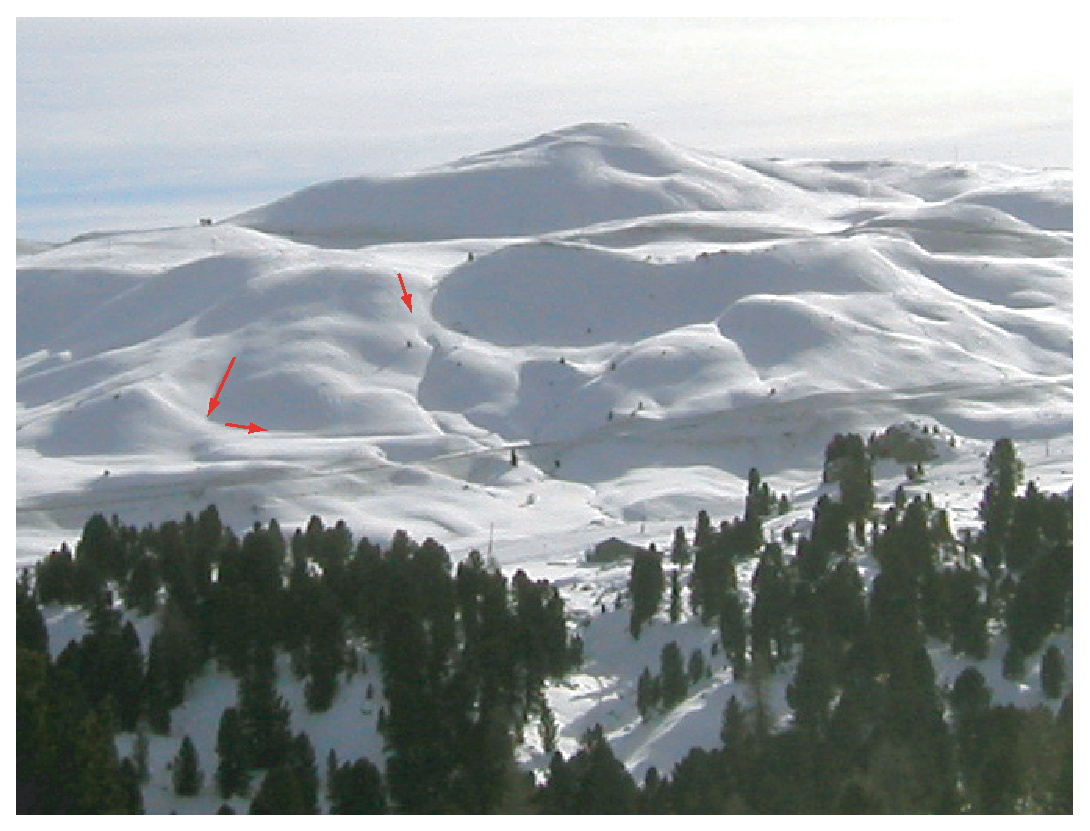
\includegraphics[width=10 cm]{EPSfiles/ski.eps}
 \caption{Illustration of the relationship between a vector field (direction and magnitude of steepest slope at every point, e.g., red arrows) and the scalar field (height) of a ski slope.}
 \label{fig:ski}
 \end{figure}
 
 
 To convert the  scalar field (height versus position) to a vector field (direction and magnitude of greatest slope) mathematically, we would simply differentiate
the topography function.   Let's say we had a  very weird two dimensional, sinusoidal
topography such that $z=f(x)=\sin x$ with $z$ the height and $x$ is the distance from some marker.  The slope in the $x$ direction ($\hat x$), then would be ${\hat x }{d \over {d x}}{ f(x) }$.  If $f(x,y,z) $ were a three
dimentional topography then the gradient of the topography function would be: 

$$
(\hat x {{\partial} \over {\partial x}} f + \hat y {{\partial} \over {\partial y}} f + \hat z
{{\partial} \over {\partial z}} f) .
$$

\noindent
For short hand, we define a ``vector differential operator'' to be a vector whose components are
 
$$\nabla = (\hat x {\partial \over {\partial x}}, \hat y {\partial \over {\partial y}},
\hat z {\partial
\over {\partial z}}).$$

\noindent
This  can also be written in polar coordinates:

$$
\nabla = {\partial \over {\partial r}}, {\partial \over {r\partial \theta}}, {\partial
\over {r\sin \theta \partial \phi}}.
$$

 \begin{figure}[htb]
%\epsfxsize 8cm
\hskip 1in 
%\centering \epsffile{EPSfiles/div.eps}
\centering  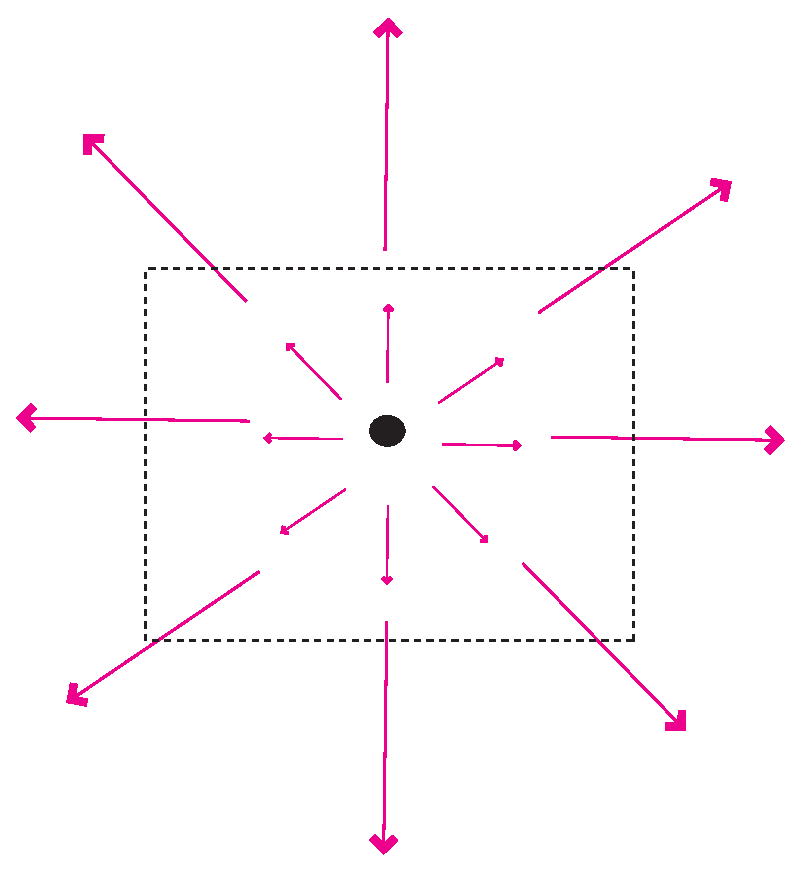
\includegraphics[width=8 cm]{EPSfiles/div.eps}
\caption{Example of a vector field with a non-zero divergence.}
\label{fig:div}
\end{figure}



\subsubsection {Divergence}

The divergence of a vector function (e.g. $\H$) is written as:

$$
\nabla \cdot \H.
$$

\noindent The trick here is to treat $\nabla$ as a vector and use  the rules for dot products described in Appendix~\ref{app:vectors}.  In
cartesian coordinates, this is:

$$
\nabla \cdot \H = \hat x {{\partial H_x} \over {\partial x}} + \hat y {{\partial H_y}\over
{\partial y}} + \hat z {{\partial H_z}\over {\partial z}}.
$$

\noindent Like all dot products, the divergence of a vector function is a scalar.
 \begin{figure}[htb]
%\epsfysize 6cm
\hskip 1in
%\centering \epsffile{EPSfiles/divzero.eps}
\centering  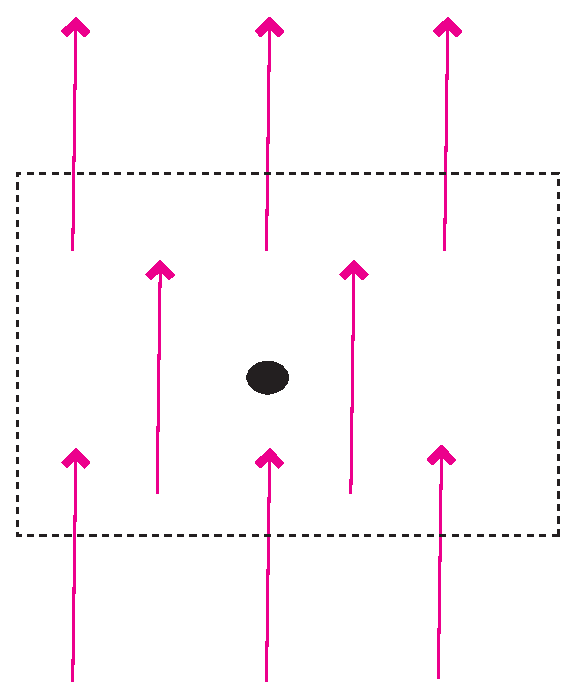
\includegraphics[width=6 cm]{EPSfiles/divzero.eps}
\caption{Example of a vector field with zero divergence.}
\label{fig:divzero}
\end{figure}
 \begin{figure}[htb]
%\epsfxsize 8cm
\hskip 1in
%\centering \epsffile{EPSfiles/curl.eps}
\centering  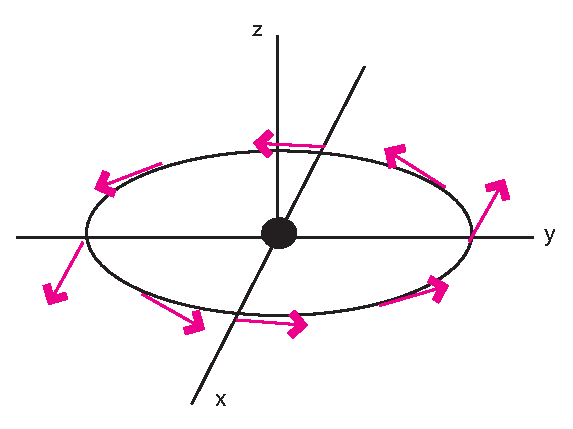
\includegraphics[width=8 cm]{EPSfiles/curl.eps}
\caption{Example of a vector field with non-zero curl.}
\label{fig:curl}
\end{figure}


The name divergence is well chosen because $\nabla \cdot \H$ is a measure of how much the
vector field ``spreads out'' (diverges) from the point in question.  In fact, what divergence quantifies is the balance between vectors coming in to a particular region versus those that go out.  
The example in  Figure~\ref{fig:div} depicts a vector function whereby the magnitude of the
vector increases linearly with distance away from the central point.  An example of such a
function would be $v(r)=r$.  The divergence of this function is:
$$
\nabla \cdot v = {\partial \over {\partial r}} r = 1.
$$
\noindent (a scalar).   There are no arrows returning in to the dashed box, only vectors going out and the non-zero divergence quantifies this net flux out of the box. 




Now consider Figure~\ref{fig:divzero}, which depicts a vector function that is constant over
space, i.e. $v(r) = k$.  The divergence of this function is:

$$
\nabla \cdot v = {\partial \over {\partial r}} k = 0.
$$

The zero divergence means that for every vector leaving the box, there is an equal and opposite vector coming in.  Put another way, no net flux results in a zero divergence.  
The fact that the divergence of the magnetic field  is zero  means that
there are no point sources (monopoles), as opposed to electrical fields that have divergence related to the
presence of electrons or protons.  

\subsubsection{Curl}

The curl of the vector function $\B$ is defined as  $\nabla \cross \B $.  
In cartesian coordinates we have

$$
\nabla \cross \B = \hat x ({\partial \over {\partial y}} B_z - {\partial \over {\partial z}}
B_y) + \hat y ({\partial \over {\partial z}} B_x - {\partial \over {\partial x}}
B_z) + \hat z ({\partial \over {\partial x}} B_y - {\partial \over {\partial y}}
B_x).$$

\noindent Curl is a measure of how much the vector function ``curls'' around a given
point.  The function describing the velocity of water in a whirlpool has a significant curl,
while that of a smoothly flowing stream does not.  



Consider Figure~\ref{fig:curl} which depicts a vector function $v=-y\hat x + x\hat y$.  The
curl of this function is:

$$
\nabla \cross \ v = \det \left|\, \matrix{
\hat x & \hat y &\hat z \cr
{\partial \over {\partial x}} & {\partial \over {\partial y}} & {\partial \over {\partial
z}}\cr 
-y & x & 0\cr}\right|, 
$$

or
$$
\hat x ( {\partial \over {\partial y}}  0 - {\partial \over {\partial z}} x ) +
\hat y ( {\partial \over {\partial x}}  0 - {\partial \over {\partial z}} (-y) ) +
\hat z ( {\partial \over {\partial x}} x - {\partial \over {\partial y}} (-y) ).
$$
$$
= 0 \hat x + 0  \hat y + 2\hat z
$$
So there is a positive curl in this function and the curl  is a vector in the $\hat z$ direction.

The magnetic field has a non-zero curl in the presence of currents or changing electric
fields.  In free space, away from currents (lightning!!), the magnetic field has zero
curl.  




\subsection{The statistical bootstrap}
\label{app:bootstrap}

Sometimes things just are not normal.  Statistically that is.  When you can not assume that your data follow some known distribution, like the normal distribution, or the Fisher distribution, what do you do?  In this section, we outline a technique called the bootstrap, which allows us to make statistical inferences when parametric assumptions fail.   The reader should also refer to Efron and Tibshirani (1993) for a more complete discussion.  \nocite{efron93}

In Figure~\ref{fig:bootstrap}, we illustrate the essentials of the
statistical bootstrap. We will develop the technique using data drawn
from a normal
distribution. First, we generate a synthetic data set by
drawing 500 data points from a normal distribution with a mean $\bar x$
 of 10 and
a standard deviation $\sigma$ of 2.  
The synthetic  data are plotted as a histogram in 
Figure~\ref{fig:bootstrap}a.  In  Figure~\ref{fig:bootstrap}b we plot
the data as a Q-Q plot (see Appendix~\ref{app:qq}) against the $z_i$ expected for  a normal distribution.   


\begin{figure}[htb]
%\epsfxsize 11cm
%\centering \epsffile{EPSfiles/bootstrap.eps}
\centering  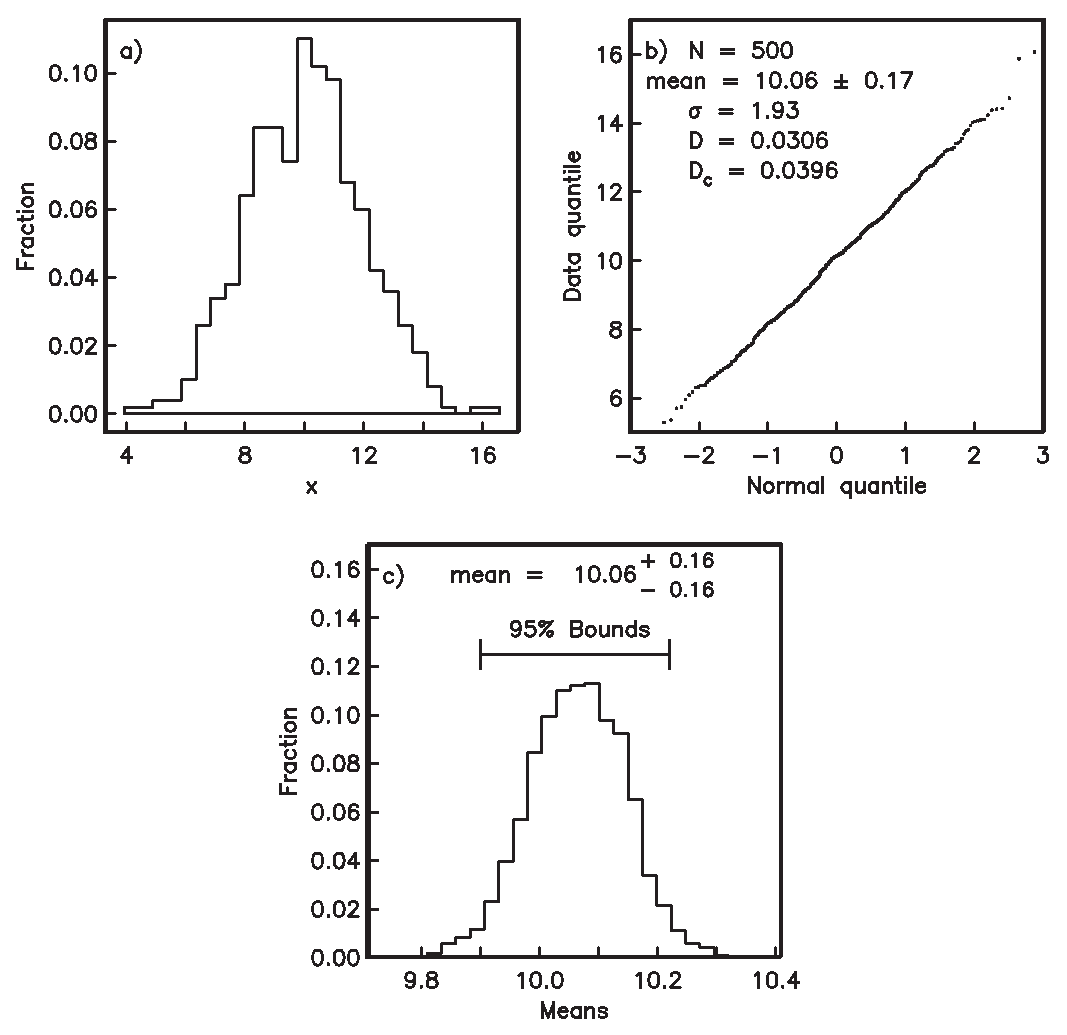
\includegraphics[width=11 cm]{EPSfiles/bootstrap.eps}
\caption { Bootstrapping applied to a normal distribution.  a)
500 data points are drawn from a Gaussian distribution with mean of
10 and a standard deviation of 2.  b) Q-Q plot of data in a). 
The 95\% confidence
interval for the mean is given by Gauss statistics as
$\pm$ 0.17.
10,000 new (para) data sets are generated by randomly drawing
$N$ data points from the original data set shown in a).  c) A
histogram of the means from all the para-data sets.  95\% of the means fall
within the interval 10.06$^{+0.16}_{-0.16}$, hence the bootstrap
confidence interval is similar to that calculated with Gaussian
statistics.  [Figure from Tauxe, 1998.]}
\label{fig:bootstrap}
\end{figure}


The data in Figure~\ref{fig:bootstrap}a plot in a line on the Q-Q plot (Figure~\ref{fig:bootstrap}b).  The value for 
$D$ is  0.0306.  Because $N=500$, the critical value of $D$, $D_c$ at the
95\% confidence level is 0.0396.  
Happily, 
our normal distribution simulation program has produced a  set of
500 numbers for which the null hypothesis of a normal distribution
has not been rejected.  
 The mean of the synthetic dataset 
is about 10 and the standard deviation is 1.9.  The usual
Gaussian statistics allow us to estimate a 95\% confidence interval for
the mean as $\pm 1.96 \sigma / \sqrt{N}$ or $\pm 0.17$. 

\begin{figure}[htb]
%\epsfysize 3in
 %\centering \epsffile{EPSfiles/sundefs.eps}
\centering  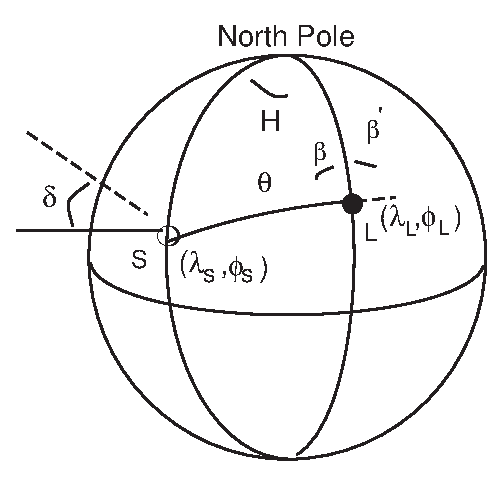
\includegraphics[width=3 in]{EPSfiles/sundefs.eps}
\caption{Calculation of the azimuth  of the shadow direction ($\beta'$)
 relative to true North, using a sun compass. L is the site location (at
$\lambda_L,\phi_L$), S is the position on the Earth where the sun is
directly overhead ($\lambda_S,\phi_S$). [Figure from Tauxe, 1998.]}
\label{fig:sundefs}
\end{figure}

In order to estimate a confidence interval for the mean using the
bootstrap, we first randomly draw a list of $N$ data by selecting data
points from the original data set.   This list is called a {\it pseudo-sample} of the data. 
Some data points will be used
more than once and others will not be used at all.  We then calculate the mean of the 
pseudo-sample.   We repeat the procedure of drawing 
pseudo-samples and calculating the mean many times (say 10,000 times).  
A histogram of the  ``bootstrapped'' means is plotted in Figure~\ref{fig:bootstrap}c. 
If these are sorted such that the first mean is the lowest
and the last mean is the highest, the 95\% of the means are  between the 250$^{th}$ and the 9,750$^{th}$
mean.   These therefore are the 95\% confidence bounds because we are approximately 95\% confident that the true mean lies between these limits.  
The 95\% confidence interval calculated for the data in 
Figure~\ref{fig:bootstrap} by bootstrap is 
about $\pm$ 0.16 which is nearly the same as that calculated the 
Gaussian way.  However, the
bootstrap required  orders of magnitude more calculations than the
Gaussian method, hence it is ill-advised to perform a bootstrap
calculation when a parametric one will do.   Nonetheless, if the data
are not Gaussian, the bootstrap provides a means of calculating
confidence intervals when there is no quick and easy way.
Furthermore, with a modern computer, the time required to calculate the bootstrap 
illustrated in Figure~\ref{fig:bootstrap} was virtually imperceptible.  

\subsection{Directions using a sun compass}
\label{app:sundec}

In a sun compass problem, we have the direction of the sun's shadow and an angle between that and the desired direction ($\alpha$).
The declination of the shadow itself 
is 180$^{\circ}$ from the direction toward the sun.  In
Figure~\ref{fig:sundefs}, the problem of calculating declination from
sun compass information is set up as a 
spherical trigonometry problem, similar to those introduced in Chapter 2 and Appendix~\ref{app:strig}.   The declination of the shadow 
direction $\beta'$, is given by  180 - $\beta$. We also  know the 
latitude of the sampling location L ($\lambda_L$).  We 
 need to calculate the latitude
of S (the point on the Earth's surface where the sun is directly
overhead),  and the local hour angle $H$.  

Knowing the time of observation (in Universal Time),
the position of S ($\lambda_s = \delta,\phi_s$ in
Figure~\ref{fig:sundefs})
can be calculated with reasonable precision (to within 0.01$^{\circ}$)
 for the period of time between 1950 and 2050 using the
procedure recommended in the 1996 Astronomical Almanac:


\begin{enumerate}

\item  First, calculate the Julian Day $J$.  
  Then, calculate the fraction of
the day in Universal Time $U$.  Finally, calculate the parameter
$d$ which is the number of days from J2000 by:

$$ d= J - 2451545 + U.$$

\item The mean longitude of the sun ($\phi_s$), corrected for
aberration, can be estimated in degrees by:

$$ \phi_s=280.461 + 0.9856474 d. $$

\item The mean anomaly $g=357.528 + 0.9856003 d$ (in degrees).

\item Put $\phi_s$ and $g$ in the range 0 $\rightarrow$ 360$^{\circ}$.

\item  The longitude of the ecliptic is given by $\phi_E=\phi_s +
1.915 \sin g + 0.020 \sin 2g$ (in degrees).

\item  The obliquity of the ecliptic is given by $\epsilon =
23.439 - 0.0000004 d$.

\item  Calculate the right ascension ($A$) by:

$$
A = \phi_E - ft \sin 2\phi_E + (f/2) t^2 \sin 4 \phi_E,
$$
\noindent where $f=180/\pi$ and $t=$tan$^2\epsilon/2$.

\item  The so-called ``declination'' of the  sun 
($\delta$ in Figure~\ref{fig:sundefs}
which should not be confused with the magnetic declination $D$),
  which we will use
as the latitude $\lambda_s$, is given by:

$$
\delta = \sin^{-1}(\sin \epsilon \sin \phi_e).
$$

\item  Finally, the equation of time in degrees is given by $E=
4(\phi_s-A)$.  

\end{enumerate}


We can now calculate the 
Greenwich Hour Angle $GHA$
from the 
Universal Time $U$ (in minutes) by $GHA = (U + E)/4 + 180$.  
The local hour angle ($H$ in Figure~\ref{fig:sundefs}) is $GHA +
\phi_L$.   We calculate $\beta$ using the laws of 
spherical trigonometry (see Appendix~\ref{app:strig}).  First we calculate $\theta$ by the Law of
Cosines (remembering that the cosine of the colatitude equals the sine
of the latitude):

$$
\cos \theta = \sin \lambda_L \sin \lambda_s + \cos \lambda_L \cos,
\lambda_s \cos H
$$

\noindent and finally using the Law of Sines:

$$
\sin \beta = (\cos \lambda_s \sin H)/\sin \theta.
$$

If $\lambda_s<\lambda_L$, then the required angle is the shadow
direction $\beta'$,
given by: $\beta' =180-\beta$.  The azimuth of the desired direction
 is $\beta'$ plus the measured shadow angle
$\alpha$. 



%\customlink{Plots_useful_in_paleomagnetism}
\chapter{Plots useful in paleomagnetism}
\section{Equal area projections}
\label{app:eqarea}


\subsection{Calculation of an equal area projection}
%\customlink{equal_area} % Lori don't change this

\begin{figure}[htb]
%\epsfxsize 10cm  
%\centering \epsffile{EPSfiles/mkeq.eps}
\centering  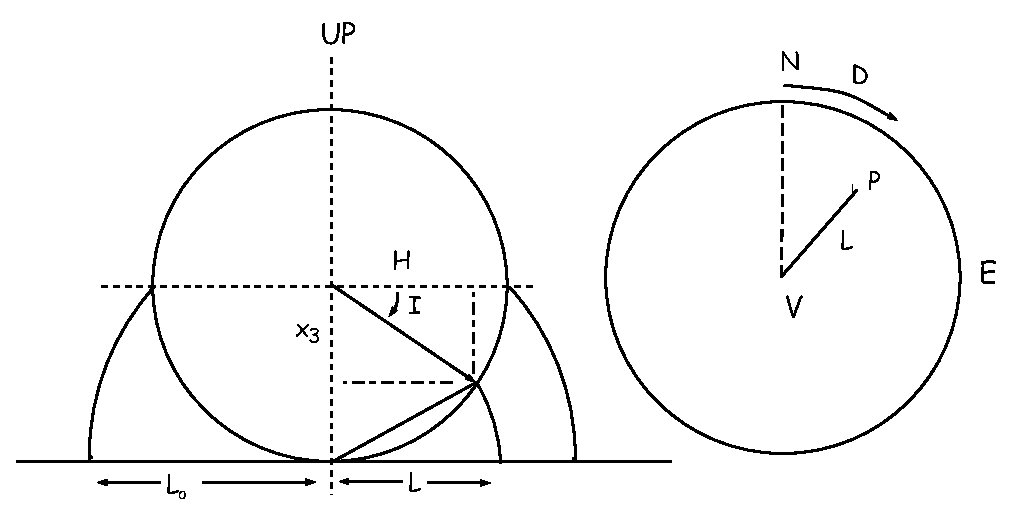
\includegraphics[width=10 cm]{EPSfiles/mkeq.eps}
\caption
{Construction of an equal area projection for a point P
corresponding to a $D$ of 40$^{\circ}$ and an $I$ of 35$^{\circ}$. [Figure from Tauxe, 1998.]}
\label{fig:mkeq}
\end{figure}

The principles for how to make an equal area projection are  shown in Figure~\ref{fig:mkeq}.
 The point P corresponds to a $D$ of 40$^{\circ}$ 
and $I$ of 35$^{\circ}$.  $D$ is measured around the
perimeter of the equal area net  and $I$ is transformed
as follows: 

\beq
L=L_o\sqrt{(1-|x_3|)},
\eeq
where $L_o = 1/\sqrt{x_1^2+x_2^2}$. 


\begin{figure}
%\epsfxsize 14cm
%\centering \epsffile{EPSfiles/equal.eps}
\centering  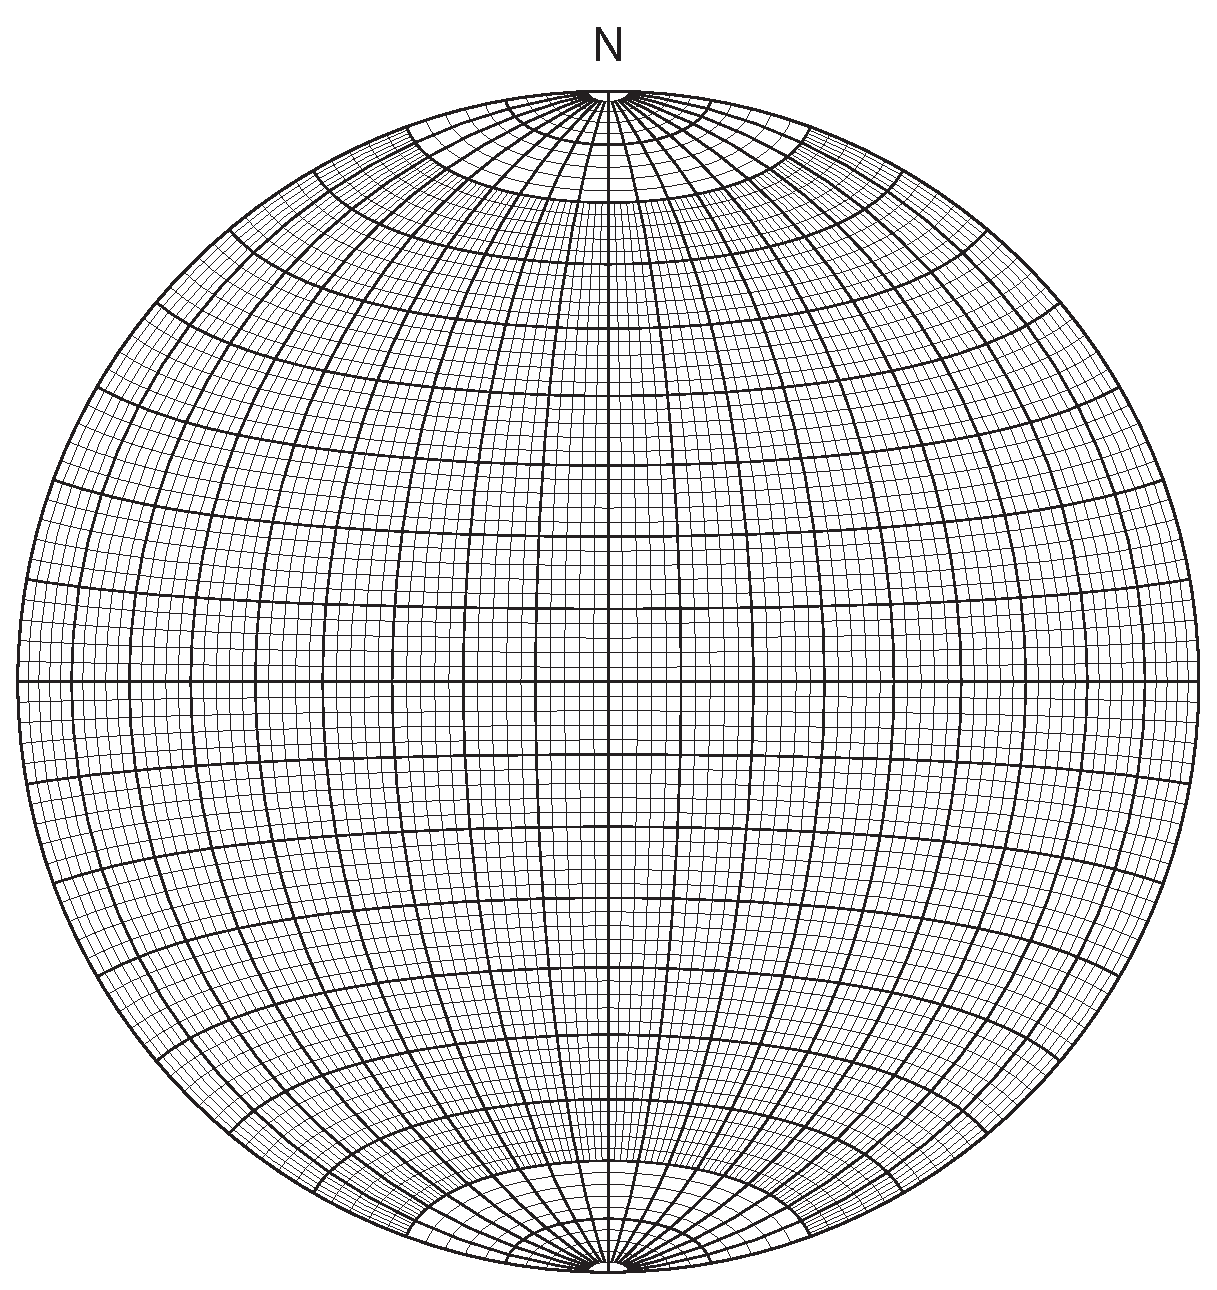
\includegraphics[width=14 cm]{EPSfiles/equal.eps}
\caption{Schmidt (equal area) net.}
\label{fig:equal}
\end{figure}


\clearpage

\begin{figure}[h!tb]
%\epsfxsize 14cm
%\centering \epsffile{EPSfiles/how2eq.eps}
\centering  \includegraphics[width=14 cm]{EPSfiles/how2eq.eps}
\caption{How to use an equal area net (see text).  }
\label{fig:how2eq}
\end{figure}

\subsection{Plotting directions}
\label{app:eqdir}

\index{diagrams!equal area}
The principles for plotting directions on an equal area net are shown in Figure~\ref{fig:how2eq}.  Print out the equal area net provided in Figure~\ref{fig:equal}.   Then poke a thumbtack through the center of the diagram and place a piece of tracing paper over the thumbtack.   Mark the top of the stereonet as N and the declination of the direction at  $Dir$ in Figure~\ref{fig:how2eq}a.  Then rotate the mark around the thumbtack  such that the declination is at the top of the diagram (Figure~\ref{fig:how2eq}b).  Count in from the outer ring the number of degrees equal to the inclination - the grid  provided is in 2$^{\circ}$ intervals.  Mark the direction (star in Figure~\ref{fig:how2eq}d).  In paleomagnetism, the convention is for solid symbols to represent downward directions and open symbols to be up.


\subsection{Bedding-tilt corrections} 
\label{app:eqtilt}
%(modified from Butler, 1992) 

Performing structural corrections can also be done with an equal area net.  If samples have been collected from sites where strata have been tilted by tectonic disturbance, a bedding tilt
correction is required to determine the NRM direction with respect to paleohorizontal. Structural attitude
of beds at the collecting site (strike and dip, or dip angle and direction) must be determined during the course
of field work.

The bedding-tilt correction is accomplished by rotating the NRM direction about the local strike axis by
the amount of the dip of the beds. Several examples are shown in Figure~\ref{fig:tilt}, and the reader is strongly
encouraged to follow through these examples. An intuitive appreciation of these geometrical operations will
prove invaluable in understanding many paleomagnetic techniques and applications.

Print out the  equal-area grid provided in Figure~\ref{fig:equal}.  Poke a thumb tack through the center and 
place a piece of tracing paper over it. The graphical procedure for the bedding-
tilt correction is as follows:

\begin{enumerate}

\item Bedding attitude is defined by the down-dip direction (the dip direction) and dip angle. In the
example of Figure~\ref{fig:tilt}, the dip direction is  40$^{\circ}$ and dip angle is 20$^{\circ}$. The azimuth of bedding strike
(orthogonal to down-dip direction) is defined as 90$^{\circ}$ anti-clockwise from dip direction (310$^{\circ}$ in the example
of Figure~\ref{fig:tilt}).


\begin{figure}[htb]
%\epsfxsize 14cm
%\centering \epsffile{EPSfiles/tilt.eps}
\centering  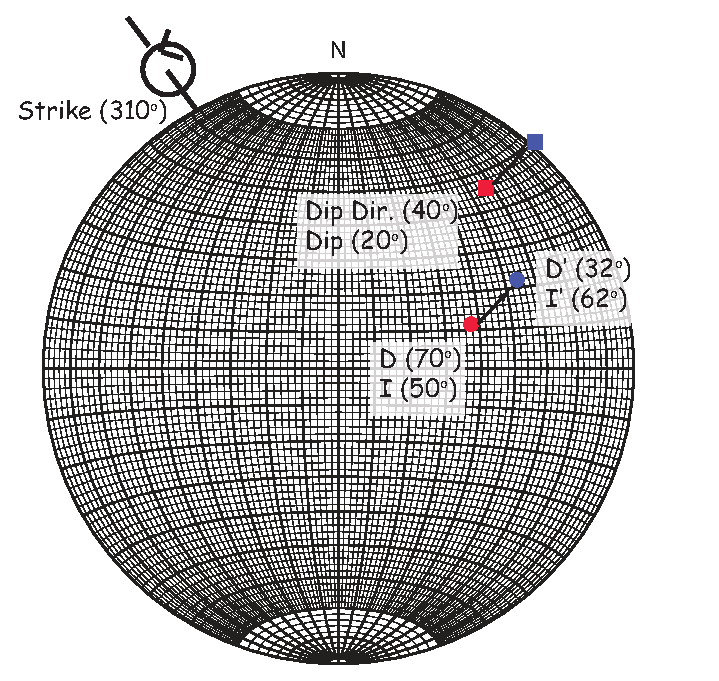
\includegraphics[width=14 cm]{EPSfiles/tilt.eps}
\caption{Example of structural corrections to NRM directions. The bedding attitude is specified by dip
and dip direction (squares on the equal-area projections); the azimuth of the strike is 90$^{\circ}$ anti-clockwise
from the dip direction; the rotation required to restore the bedding to horizontal is clockwise
(as viewed along the strike line) by the dip angle and is shown by the rotation symbol; the {\it in situ}
NRM direction is at the tail of the arrow, and the structurally corrected NRM direction is at the
head of the arrow.}
\label{fig:tilt}
\end{figure}

\clearpage



\item  Put the dip direction/ dip angle and the paleomagnetic direction on the equal area net as described in Appendix~\ref{app:eqdir}.  These should look like the red square and circle respectively in Figure~\ref{fig:tilt}.  Now mark the strike direction as shown in Figure~\ref{fig:tilt}.   Rotate the  equal-area grid such that the strike is at the top of the grid (you can also put it at the bottom or on either side).  
  
\item The NRM direction is rotated clockwise about the strike azimuth (along a small circle) by an angle
equaling the dip angle.  In practice, this means that you count degrees from the circle toward the outer rim along the nearest small circle by the amount of the dip direction.    If you reach the outer rim, just ``walk back'' in toward the center and keep counting.   Plot a new circle (the blue one) at that point.  If you reached the outer rim and continued back toward the center, this is a negative inclination (upward pointing) and you should use an open symbol.  

\item   Following this rotation, the {\it in situ} direction can be read from the equal-area
projection.  Rotate the blue dot to the up-down axis and make a mark on the outer rim.  The degrees between this mark and the $N$ marked is the new declination.  The number of degrees between the blue circle and the outer rim is the new inclination.   For the example of Figure~\ref{fig:tilt}, the {\it in situ} direction is $I$ = 50$^{\circ}$,$ D$ = 70$^{\circ}$ and the direction
corrected for bedding tilt is $I$ = 32$^{\circ}$; $D$ = 62$^{\circ}$.

\end{enumerate}


\subsection{Reading ternary diagrams}
\label{app:ternary}

\index{diagrams!ternary}
Ternary diagrams are triangles with the three corners representing a composition (e.g., A,B,C or Fe, FeO, Fe$_2$O$_3$).  In Figure~\ref{fig:how2tern}a we show only the A component.  To get the percentage of this component, we count up from the base of the triangle and find that the star is 60\% of the way toward the apex, indicating that the compound is 60\% A in composition.  The percentage of composition B is shown in Figure~\ref{fig:how2tern}b (15\%) and similarly C is shown in Figure~\ref{fig:how2tern}c (25\%).    



\begin{figure}[htb]
%\epsfxsize 14cm
%\centering \epsffile{EPSfiles/ternary.eps}
\centering  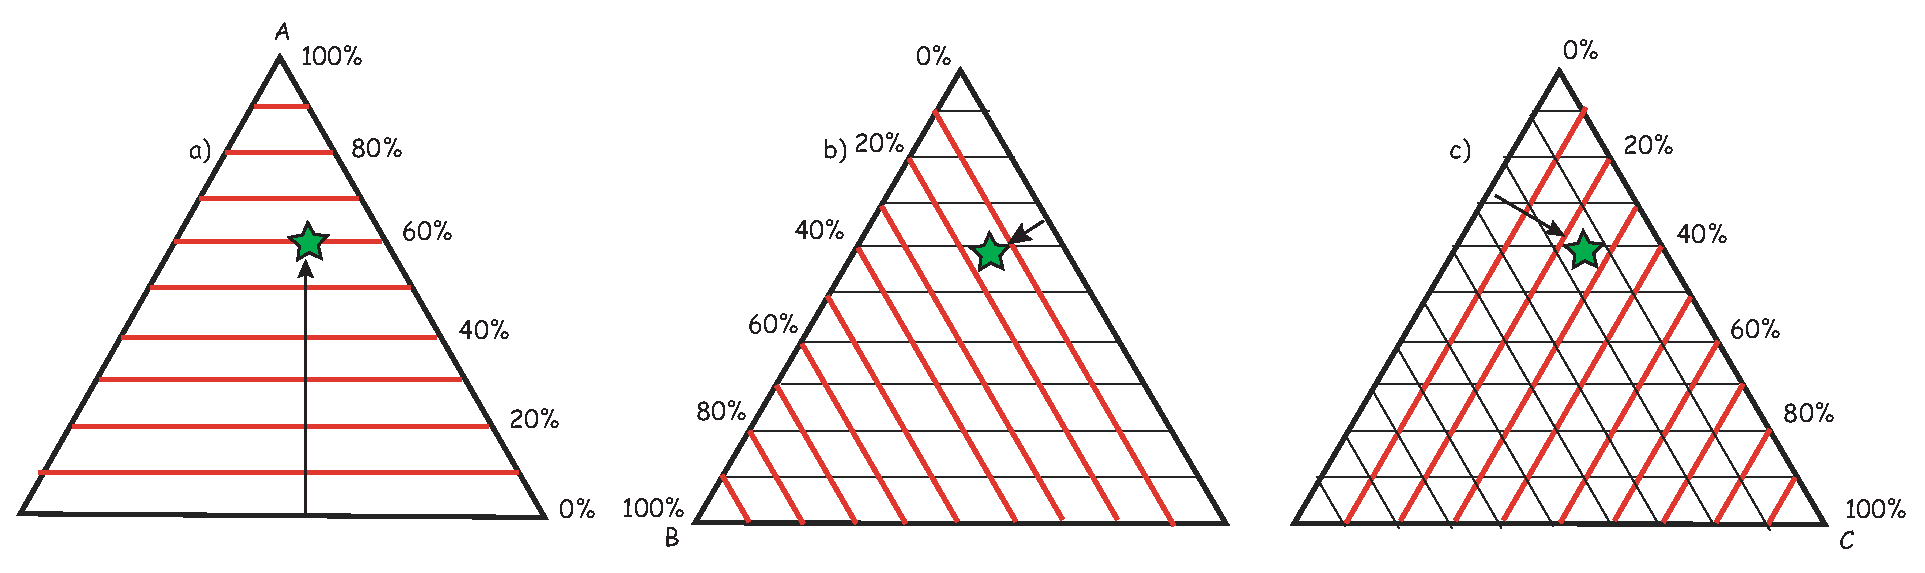
\includegraphics[width=14 cm]{EPSfiles/ternary.eps}
\caption{How to read a ternary diagram.  The three apices are components A,B,C.  A composition is plotted as the star.  a) Shows the percentage of component A (60\%).  b) Shows the percentage of component B (15\%) and c) shows the percentage of component C (25\%).  }
\label{fig:how2tern}
\end{figure}  

%\customlink{quantile_quantile_plots}
\subsection{Quantile-Quantile plots}
\label{app:qq}

When does a data set conform to a particular distribution?   One way to assess this is through the use of
\index{diagrams!quantile-quantile}
{\it Quantile-quantile}, or Q-Q, plots (see 
\index{Fisher, N.I.}
Fisher et al., 1987 for a more complete discussion.)  In a Q-Q plot, data are graphed against the value expected from a particular distribution. The data $\zeta_i$ are plotted against a value $z_i$ that is expected from the distribution; data compatible  with the chosen distribution plot along a line.   First, we will develop the Q-Q plot for the uniform and exponential functions required for a Fisher distribution.  Then we will explain how make a Q-Q plot for a normal distribution.  

\begin{figure}[h!tb]
%\epsfxsize 12cm
%\centering \epsffile{EPSfiles/Ais.epsf}
\centering  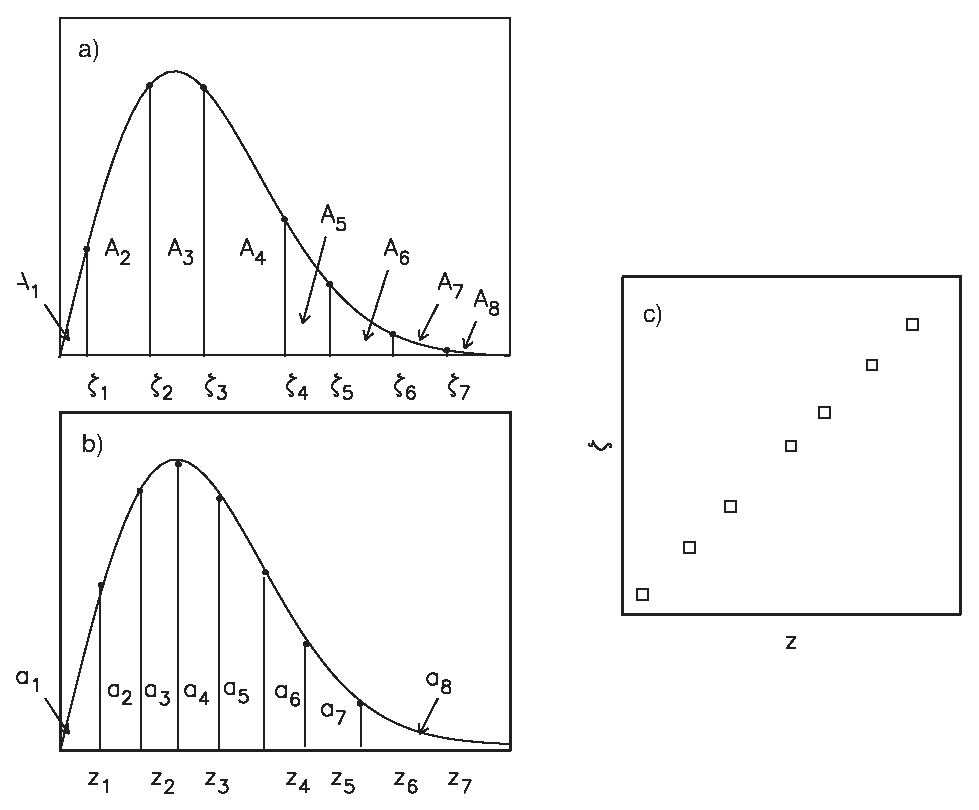
\includegraphics[width=12 cm]{EPSfiles/Ais.eps}
\caption{
a) Illustration of how the sorted data $\zeta_i$ divide the density curve into
areas $A_i$ with an average area of $1/(N+1)$. b) The values of $z_i$ which
divide the density function into equal areas $a_i=1/(N+1)$.  c) Q-Q plot of
$z$ and $\zeta$. [Figure from Tauxe, 1998.]
}
\label{fig:Ais}
\end{figure}


\subsubsection{Q-Q plots for Fisher distributions}

In order to make Q-Q plot for Fisher distributions, we proceed as follows (Figure~\ref{fig:Ais}):


\begin{enumerate}

\item  Sort the variable of interest $\zeta_i$ into ascending order so that $\zeta_1$
is the smallest and $\zeta_N$ is the largest. 

\item  If the data are represented by the underlying density function as
in Figure~\ref{fig:Ais}a, then the $\zeta_i$'s divide the curve into
$(N+1)$ areas, $A_i$, the average value of which is $a=1/(N+1)$. If we assume a
form for the density function of $\zeta_i$, we can calculate numbers $z_i$, that
divide the theoretical distribution into areas $a_i$ each having an area 
$a$ (see Figure~\ref{fig:Ais}b). 

\item  An approximate test for whether the data $\zeta_i$ are fit by a given
distribution is to plot the pairs of points ($\zeta_i, z_i$), as shown in
Figure~\ref{fig:Ais}c.  If the assumed
distribution is appropriate, the data will plot as a straight line. 

\item  The density function $P$ is the distribution function $F$ times the area,
as mentioned before.  The $z_i$ are calculated as follows:
\begin{equation}
F(z_i)=(i-\half)/n, \hbox{where }i=1,\dots,n,
\label{eq:Fz}
\end{equation}
\noindent
so that:
\begin{equation}
z_i=F^{-1}((i-\half)/n), \hbox{where } i=1,\dots,n,
\label{eq:zi}
\end{equation}
and where $F^{-1}$ is the inverse function to $F$.  If the data are uniformly
distributed (and constrained to lie between 0 and 1), then both $F(x)$ and  $F^{-1}(x) =x $.
  For an exponential distribution
$F(x)=1- e^{-x}$ and
$F^{-1}(x)=-\hbox{ln}(1-x)$. 

\item  Finally,  we can calculate parameters $M_u$ and $M_e$ which, when compared
to critical values, allow rejection of
the hypotheses of uniform and exponential distributions, respectively. 
To do this, we first calculate:
\begin{equation}
D_N^+ = \hbox {maximum} [{i\over N} - F(x)],
\label{eq:DNp}
\end{equation}
and
\begin{equation}
D_N^- = \hbox {maximum} [F(x) -{{(i-1)}\over N} ].
\label{eq:DNn}
\end{equation}
For a uniform distribution $F(x)=x$, so
 $M_u$ is calculated by first calculating $D_N^+$ as the maximum
of $[i/N-\zeta_i]$ and $D_N^-$ as the maximum of $[\zeta_i-(i-1)/N]$. The Kuiper's  statistic $V_n$
is $D_N^++D_N^-$ and $M_u$ is given by:

\begin{equation}
M_u = V_n (\sqrt{N} - 0.567 + {1.623\over{\sqrt{N}}}), 
\label{eq:Mu}
\end{equation}

\noindent (see 
\index{Fisher, N.I.}
Fisher et al.,  1987).   A value of $M_u > 1.207$  
 can be grounds for rejecting the
hypothesis of uniformity at the 95\% level of certainty.
 Similarly,  $D_N^+$ and $D_N^-$  can be calculated for the
inclination data (using $\zeta_i=90-I_i$) as  $[i/N-(1-e^{-\zeta_i})]$
and maximum of $[(1-e^{-\zeta_i})-(i-1)/N]$ respectively.   The Kolmogorov-Smirnov statistic $D_n$ is  the largest of the two.   The test statistic for exponentially distributed data  $M_e$ is given by:

\begin{equation}
M_e = {(D_n - {0.2 \over{N}})} {( \sqrt N + 0.26 + {1\over {2\sqrt N} } )}.
\label{eq:Me}
\end{equation}

\noindent Values of $M_e$ larger than 1.094 allow rejection of the exponential
hypothesis at the 95\% level of confidence.   If either $M_u$
or $M_e$ exceed the critical values, the hypothesis of a Fisher distribution
can be rejected. 
\end{enumerate}

\subsubsection{Q-Q plots for normal distributions}

In order to calculate the appropriate values for $z_i$ assuming a normal
distribution (see Abramowitz and Stegun, 1970):  

\begin{enumerate}

\item For $i=1\rightarrow N$, calculate $p = {i\over {N+1}}$.
\item  If $p>0.5$, then $q=1-p$; if $p<0.5$, then $q=p$.  

\item  Calculate the following for all $p\ne 0.5$:

$$t=\sqrt{-2\logn^{-1}(q)},$$

and 

$$
u=t-{ {(a_1+a_2t_+a_3t^2)}\over { (1 +a_4t+a_5t^2+a_6t^3)}},
$$
\noindent where $a_1=2.515517,
a_2=0.802853,a_3=0.010328,a_4=1.432788,a_5=0.189269,a_6=0.001388$.  

\item  If $p>0.5$, then $z_i=u$; if $p<0.5$, then $p=-u$.

\item  If $p=0.5$, then $z_i=0$.  
\end{enumerate}

The values of $z_i$ calculated in this way for a simulated Gaussian
distribution are plotted as the ``normal quantile'' data and will plot along a line if the data are in fact normally distributed.
 To test this in a more quantitative way,
we can calculate $D_N^+$ and $D_N^-$ as follows:  

\begin{enumerate}

\item Calculate the mean $\bar x$ and standard deviation $\sigma$ for the
data.

\item  Then calculate:
$${p=} {{x_i - \bar x}\over {\sqrt 2 \sigma}},$$

\noindent and

$${q =} {1\over {1+{0.3275911|x|}}}.$$  

\item  Substitute $q$ into the following expression (function 7.1.26 from
\index{Abramowitz, M.}%
\index{Stegun, I.}%
Abramowitz and Stegun, 1970): 

$$
\erf(q) = 1-e^{-p^2} [ a_1q +a_2q^2 + a_3 q^3 + a_4 q^4+a_5q^5],
$$
\noindent where $a_1=0.254829592,a_2=-0.284496736,a_3=1.421413741,$ and
$a_5= 1.061405429$.

\item  Change the sign of $\erf(q)$ such that it has the same sign as $q$.

\item  Substitute $F(x)=0.5(1+\erf(q))$ into Equations   and 
~\ref{eq:DNn}  in Appendix~\ref{app:qq}  for
$D_N^+$ and $D_N^-$ respectively.  The Kolmogorov-Smirnov
 parameter $D$ (e.g., 
\index{Fisher, N.I.}%
Fisher et al., 1987) is the larger of $D_N^+$ or $D_N^-$.  

\item  The null hypothesis that a given data set is normally distributed can
be rejected at the 95\% level of confidence if $D$ exceeds a critical
value $D_c$ given by $0.886/\sqrt{N}$.
\end{enumerate}



%\customlink{Paleomagnetic_statistics_and_parameter_estimation}
\chapter {Paleomagnetic statistics and parameter estimation}  


Chapters 5 and 7  discussed various hysteresis parameters and Chapters 11 and 12 developed the major features of paleomagnetic directional statistics.  Here we go over some aspects in greater detail.   

%\customlink{hysteresis_parameters}
\section{Hysteresis Parameters}
\label{app:hyst}


\index{hysteresis!parameter estimation}
A typical hysteresis experiment involves determination of a hysteresis loop and frequently also a back-field curve (see Figure~\ref{fig:hparcalc}).    Processing of the data in the {\bf PmagPy} software package (see, e.g.,  Example for {\bf hysteresis\_magic.py}) proceeds as follows:

\begin{enumerate}
\item Sometimes the descending and ascending hysteresis loops do not close because of instrument drift (see Figure~\ref{fig:hparcalc}a).  Ordinarily, the experiment should be re-done,  but for small differences, we force the loops to  close  by subtracting the difference, interpolated from the maximum difference at the maximum field ($B_{max}$) to a zero difference at the minimum field ($B_{min}$).    
\item  After closing the loops, we calculate the best-fit line to the $M, B$ data for  the portion within 70\% of $\pm B_{max}$, averaging data from both the ascending and descending loops.  A difference in the absolute value of the y-intercepts for the ascending and descending loops indicates a vertical offset of the data, which is adjusted such that the two intercepts are equal.  The average slope is the high-field susceptibility ($\chi_{hf}$), which is subtracted off.  The data after these steps are shown as the dashed line in Figure~\ref{fig:hparcalc}.  The maximum magnetization after adjusting for the 
\index{magnetic!susceptibility!high field}
$\chi_{hf}$ is the 
\index{magnetization!saturation}
saturation magnetization $M_s$.  


\begin{center}
  \begin{table}[htb]
  \caption{Summary of hysteresis parameters.}
  \label{tab:hystpars}
  \begin{tabular}{llll}
  \hline
  Symbol&Method & Section&Figure\\
  \hline
$\chi_{hf}$&high field susceptibility&~\ref{sect:chi} \&~\ref{sect:hyst}&~\ref{fig:Bcr} \& ~\ref{fig:hparcalc}\\
  $M_s$&saturation magnetization& ~\ref{sect:para}&~\ref{fig:Bcr} \& ~\ref{fig:hparcalc}\\ 
 $M_r$&saturation remanence& ~\ref{sect:uniaxial} \&~\ref{sect:irm}&~\ref{fig:Bcr} \& ~\ref{fig:hparcalc}\\ 
$H_{c}$ or $\mu_oH_{c}$  & Coercivity & ~\ref{sect:K1} \& ~\ref{sect:uniaxial}&\ref{fig:Bcr} \& ~\ref{fig:hparcalc}\\
\multicolumn{3}{l} {Coercivity of remanence:}\\
  $H_{cr}$&$\Delta M$ method& ~\ref{sect:uniaxial}& ~\ref{fig:hparcalc}\\
$H_{cr}'$ &ascending loop intercept method& ~\ref{sect:uniaxial}&~\ref{fig:Bcr}\\
$H_{cr}''$ &Back-field method&~\ref{sect:irm}, &~\ref{fig:irm} \&~\ref{fig:hparcalc}\\
$H_{cr}'''$&$ H_{1/2}$ method&~\ref{sect:irm} \& \ref{sect:unmixing}&~\ref{fig:irm} \& ~\ref{fig:unmixing}\\
\hline
\end{tabular}
\end{table}
\end{center}


\begin{figure}[htb]
%\epsfxsize 12cm
%\centering \epsffile{EPSfiles/hparcalc.eps}
\centering  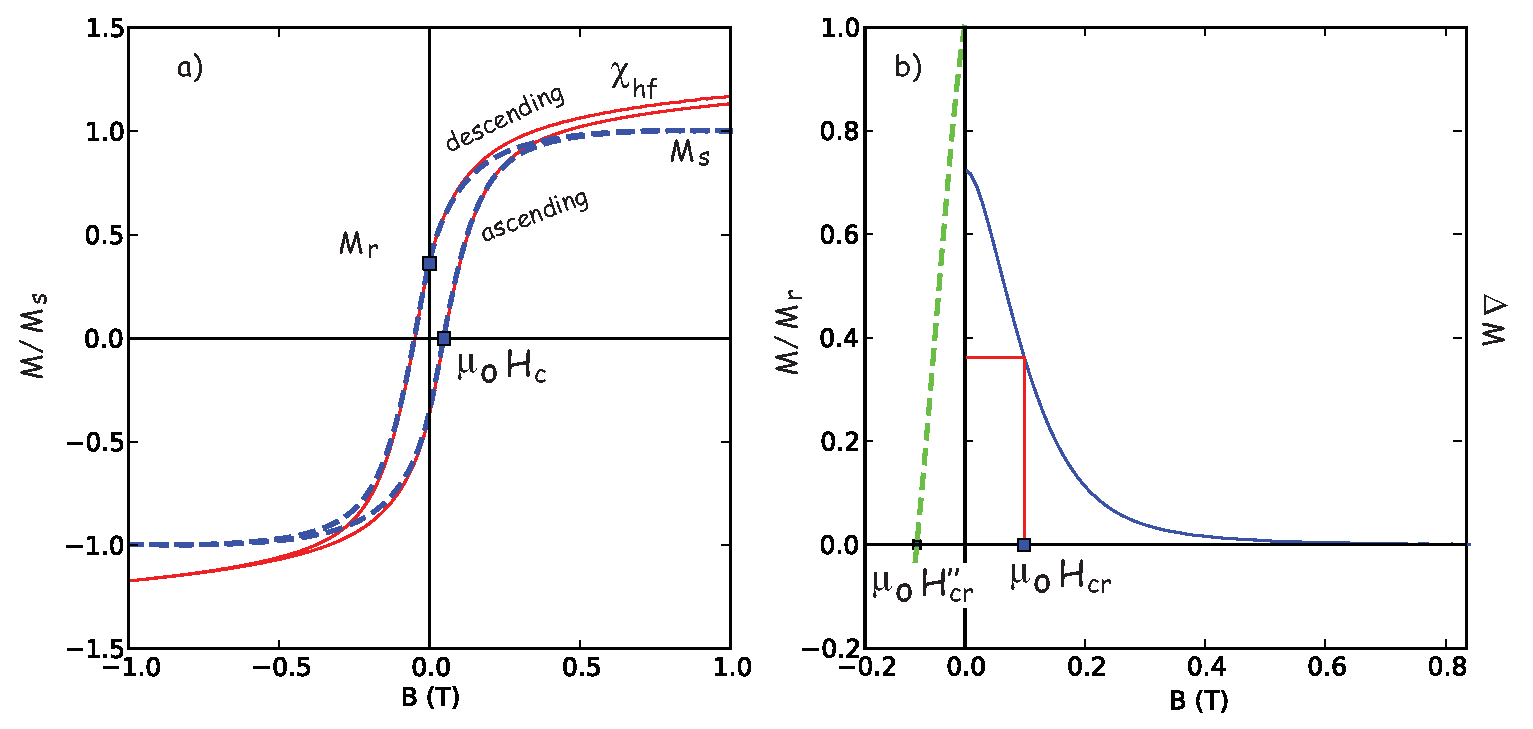
\includegraphics[width=12 cm]{EPSfiles/hparcalc.eps}
\caption{Typical hysteresis experiment.  a)  Raw data are solid red line.  Data are processed (see text) by closing the ascending and descending loops, subtracting the high field slope ($\chi_{hf}$) and adjusting such that the y-intercepts are equal (that for the descending loop is labeled $M_r$).   Processed data  are dotted blue line. Coercivity ($\mu_oH_{c}$) is the applied field for which a saturation magnetization ($M_s$) is reduced to zero.        b) Difference between processed ascending and descending loops is the $\Delta M$ curve (solid blue line).  Back-field IRM data shown normalized by saturation remanence ($M_r$)  --  dashed green line.  Two methods of estimating coercivity of remanence shown (see text).}
\label{fig:hparcalc}
\end{figure}
\clearpage



\item Coercivity ($\mu_o H_c$) is the field at which  $M=0$.   We estimate this by finding the values of $B$ between which $M$ switches sign for both the ascending and descending loops (after adjustment), calculate a line and evaluate the  $B$ for which $M=0$.  The coercivity is the average of the two estimates.  
\item   We fit a spline to the adjusted ascending and descending loops and resample the loops at even intervals of $B$ (usually 10 mT intervals).  The $\Delta M$ curve shown in Figure~\ref{fig:hparcalc}b is the difference between these two interpolated curves, averaging the data for negative and positive $B$.   The saturation remanence $M_r$ is the value of the $\Delta M$ curve at $B=0$. The coercivity of remanence ($\mu_oH_{cr}$ in Table~\ref{tab:hystpars}) is the field for which $\Delta M$ is half the value of $M_r$.  This is the ``$\Delta M$'' method of coercivity of remanence calculation (see Chapter 5).  
\item  If there are ``back-field'' IRM data as in Figure~\ref{fig:hparcalc}b, the coercivity of remanence can be estimated by finding (through interpolation) the applied field which reduces the saturation remanence ($M_r$) to zero.  This is the ``back field'' method.   

\end{enumerate}






\section{Directional statistics}
\label{app:dirstics}

\begin{table}[htb]
\begin{center}
\caption{Critical values of $R_o$ for a random distribution
 [Watson, 1956.]}
 \label{tab:Ro}
\begin{tabular}{rrr|rrr}
\hline
$N$&95\%&99\%& N&95\%&99\%\\
\hline
5 & 3.50& 4.02& 13 & 5.75& 6.84\\
6 & 3.85 & 4.48& 14 & 5.98&7.11\\
7 & 4.18 & 4.89& 15& 6.19 &7.36\\
8 & 4.48 & 5.26& 16& 6.40& 7.60\\
9 & 4.76 & 5.61& 17&6.60&7.84\\
10 & 5.03 & 5.94& 18& 6.79& 8.08\\
11 & 5.29 & 6.25& 19&6.98&8.33\\
12 & 5.52& 6.55& 20& 7.17&8.55\\
\hline
\end{tabular}
\end{center}
\end{table}



\subsection{Calculation of Watson's $V_w$}
\label{app:watsonsV}

\begin{enumerate}

\item  Calculate $R_i$, and $k_i$  where $i=1,2$ for the two data sets with $N_1, N_2$ samples using Equations~\ref{eq:R} and ~\ref{eq:k}.

\item  Calculate $\bar x_{ij}$ (where $j=1,3$ for the three axes) using Equation~\ref{eq:xbar}.
\item  Calculate $\bar X_{ij}= R_i \bar x_{ij}$.  

\item   Find the weighted means for the two data sets:

$$
\hat X_j = \sum_i^2 k_i\bar X_{ij}.
$$

\item   Calculate the  weighted overall resultant vector $R_w$ by
$$
R_w = (\hat X_1^2 + \hat X_2^2 + \hat X_3^2)^{1\over 2},
$$
\noindent   and the weighted sum $S_w$ by,
$$
S_w = \sum_i^2 k_iR_i.
$$

\item   Finally, Watson's $V_w$ is defined as
$$
V_w = 2(S_w -R_w).
$$
\end{enumerate}

%\customlink{linesNplanes}
\subsection{Combining lines and planes}
\label{app:linesNplanes}

\begin{enumerate}
\item  Calculate $M$ directed lines  (two in our case)
and $N$ great circles  (one in our case)
using principal component analysis  (see Chapter  9) or Fisher
statistics.  

\item  Assume that the primary direction of magnetization for the samples
with great circles lies somewhere along the great circle path (i.e., within the
plane).

\item  Assume that the set of $M$ directed lines and $N$ unknown
directions are drawn from a Fisher distribution.

\item  Iteratively search along the great circle paths for directions
that maximize the resultant vector $R$ for the $M+N$ directions.

\item  Having found the set of $N$ directions that lie along their respective great
circles,   estimate the mean direction using
 Equation~\ref{eq:xbar} and $\kappa$ as:

$$ 
k= {{2M+N-2}\over {2(M+N-R)}},
$$
\noindent The cone of 95\% confidence about the mean is given by:

$$
\cos \alpha_{95} = 1 - 
{ {N'-1}\over {kR}} ,
\bigl[ 
\bigl({ {1\over p}\bigr)^{1/(N'-1)}} -1
\bigr],
$$
\noindent where $N'=M+N/2$ and $p$ = .02

\end{enumerate}
{
\begin{sidewaystable}
\begin{center}
\caption{Maximum likelihood estimators of $k_1, k_2$ in the Bingham distribution for given eigenvalues $\omega_1, \omega_2$.  Data from Mardia and Zemroch (1977). Upper (lower) number is $k_1(k_2)$}
\tiny
\label{tab:bingham}
\begin{tabular}{r|rrrrrrrrrrrrrrrr}
\hline
$\omega_1$&0.02& 0.04& 0.06& 0.08& 0.10& 0.12& 0.14& 0.16& 0.18& 0.20& 0.22& 0.24& 0.26& 0.28& 0.30& 0.32 \\
\hline
$\omega_2 $\\ 
0.02&-25.55 \\
 &-25.55 \\
0.04&-25.56&-13.11 \\
 &-13.09&-13.11 \\
0.06&-25.58&-13.14&-9.043 \\
 &-8.996&-9.019&-9.043 \\
0.08&-25.6&-13.16&-9.065&-7.035 \\
 &-6.977&-6.999&-7.020&-7.035 \\
0.10&-25.62&-13.18&-9.080&-7.042&-5.797 \\
 &-5.760&-5.777&-5.791&-5.798&-5.797 \\
0.12&-25.63&-13.19&-9.087&-7.041&-5.789&-4.917 \\
 &-4.923&-4.934&-4.941&-4.941&-4.933&-4.917 \\
0.14&-25.64&-13.20&-9.087&-7.033&-5.773&-4.896&-4.231 \\
 &-4.295&-4.301&-4.301&-4.294&-4.279&-4.258&-4.231 \\
0.16&-25.65&-13.20&-9.081&-7.019&-5.752&-4.868&-4.198&-3.659 \\
 &-3.796&-3.796&-3.790&-3.777&-3.756&-3.729&-3.697&-3.659 \\
0.18&-25.65&-13.19&-9.068&-6.999&-5.726&-4.836&-4.160&-3.616&-3.160 \\
 &-3.381&-3.375&-3.363&-3.345&-3.319&-3.287&-3.249&-3.207&-3.160 \\
0.20&-25.64&-13.18&-9.05&-6.974&-5.694&-4.799&-4.118&-3.570&-3.109&-2.709 \\
 &-3.025&-3.014&-2.997&-2.973&-2.942&-2.905&-2.863&-2.816&-2.765&-2.709 \\
0.22&-25.63&-13.17&-9.027&-6.944&-5.658&-4.757&-4.071&-3.518&-3.053&-2.649&-2.289 \\
 &-2.712&-2.695&-2.673&-2.644&-2.609&-2.568&-2.521&-2.470&-2.414&-2.354&-2.289 \\
0.24&-25.61&-23.14&-8.999&-6.910&-5.618&-4.711&-4.021&-3.463&-2.993&-2.584&-2.220&-1.888 \\
 &-2.431&-2.410&-2.382&-2.349&-2.309&-2.263&-2.212&-2.157&-2.097&-2.032&-1.963&-1.888 \\
0.26&-25.59&-13.12&-8.966&-6.870&-5.573&-4.661&-3.965&-3.403&-2.928&-2.515&-2.146&-1.809&-1.497 \\
 &-2.175&-2.149&-2.117&-2.078&-2.034&-1.984&-1.929&-1.869&-1.805&-1.735&-1.661&-1.582&-1.497 \\
0.28&-25.57&-13.09&-8.928&-6.827&-5.523&-4.606&-3.906&-3.338&-2.859&-2.441&-2.066&-1.724&-1.406&-1.106 \\
 &-1.939&-1.908&-1.871&-1.828&-1.779&-1.725&-1.665&-1.601&-1.532&-1.458&-1.378&-1.294&-1.203&-1.106 \\
0.30&-25.54&-13.05&-8.886&-6.778&-5.469&-4.547&-3.842&-3.269&-2.785&-2.361&-1.981&-1.634&-1.309&-1.002&-0.708 \\
 &-1.718&-1.682&-1.641&-1.596&-1.540&-1.481&-1.417&-1.348&-1.274&-1.195&-1.110&-1.020&-0.923&-0.819&-0.708 \\
0.32&-25.50&-13.01&-8.839&-6.725&-5.411&-4.484&-3.773&-3.195&-2.706&-2.277&-1.891&-1.537&-1.206&-0.891&-0.588&-0.292 \\
 &-1.510&-1.470&-1.423&-1.371&-1.313&-1.250&-1.181&-1.108&-1.028&-0.944&-0.853&-0.756&-0.653&-0.541&-0.421&-0.292 \\
% \hline
%\end{tabular}
%\end{center}
%\end{sidewaystable}
%\clearpage
%\begin{sidewaystable}
%\begin{center}
%\tiny
%\begin{tabular}{r|rrrrrrrrrrrrrrrr}
%\hline
%$\omega_1$&0.02& 0.04& 0.06& 0.08& 0.10& 0.12& 0.14& 0.16& 0.18& 0.20& 0.22& 0.24& 0.26& 0.28& 0.30& 0.32 \\
%\hline
%$\omega_2 $\\ 
0.34&-25.46&-12.96&-8.788&-6.668&-5.348&-4.415&-3.699&-3.116&-2.621&-2.186&-1.794&-1.433&-1.094&-0.771&-0.459&-0.152 \\
 &-1.312&-1.267&-1.216&-1.159&-1.096&-1.028&-0.955&-0.876&-0.791&-0.701&-0.604&-0.500&-0.389&-0.269&-0.140&0.000 \\
0.36&-25.42&-12.91&-8.731&-6.606&-5.280&-4.342&-3.620&-3.032&-2.531&-2.089&-1.690&-1.322&-0.974&-0.642 \\
 &-1.123&-1.073&-1.017&-9.555&-0.887&-0.814&-0.736&-0.651&-0.561&-0.464&-0.360&-0.249&-0.129&0.000 \\
0.38&-25.37&-12.86&-8.670&-6.539&-5.207&-4.263&-3.536&-2.941&-2.434&-1.986&-1.579&-1.202 \\
 &-0.940&-0.885&-0.824&-0.757&-0.684&-0.606&-0.522&-0.432&-0.335&-0.231&-0.120&0.000 \\
0.40&-25.31&-12.80&-8.604&-6.466&-5.126&-4.179&-3.446&-2.845&-2.330&-1.874 \\
 &-0.762&-0.702&-0.636&-0.564&-0.486&-0.402&-0.312&-0.215&-0.111&-0.000 \\
0.42&-25.5&-12.73&-8.532&-6.388&-5.045&-4.089&-3.349&-2.741 \\
 &-0.589&-0.523&-0.452&-0.374&-0.290&-0.200&-0.104&0.000 \\
0.44&-25.19&-12.66&-8.454&-6.305&-4.955&-3.992 \\
 &-0.418&-0.347&-0.270&-0.186&-0.097&0.000 \\
0.46&-25.12&-12.58&-8.371&-6.215 \\
 &-0.250&-0.173&-0.090&0.000 \\
\hline
\end{tabular}
\end{center}
\end{sidewaystable}
}
\clearpage

\subsection{Inclination only calculation}
\label{app:incfish}

We wish to estimate the  co-inclination ($\alpha=90-I$)
 of $N$ Fisher distributed data
($\alpha_i$), the declinations of which are unknown.  
We define the estimated value of $\alpha$ to be
$\hat \alpha$.  
\index{McFadden, P.L.}%
McFadden and Reid showed that $\hat \alpha$ is the solution of:

$$
N \cos \hat \alpha + (\sin^2\hat \alpha-\cos^2\hat\alpha)\sum \cos \alpha_i -2\sin \hat \alpha
\cos \hat \alpha \sum \alpha_i = 0,
$$

\noindent
which can be solved numerically.

They further define two parameters $S$ and $C$ as:

$$
S = \sum \sin(\hat \alpha - \alpha_i),
$$
$$
C = \sum \cos(\hat \alpha - \alpha_i).
$$

An unbiassed  approximation for the Fisher parameter $\kappa$, $k$ is given by:

$$
{k =} { {N-1}\over {2(N-C)} }.
$$

The unbiased estimate $\hat I$ of the true inclination is: 

$$
\hat I= 90 - \hat \alpha + {S\over C}.
$$

Finally, the $\alpha_{95}$ is estimated by:

$$
\cos \alpha_{95} = 1 - {1\over 2}  \bigl({S\over C}\bigr)^2 - {f\over{2Ck}},
$$
\noindent
where $f$ is the critical value taken from the $F$ distribution (see F-distribution tables in statistics textbooks or online) with 1 and ($N$-1) degrees
of freedom.





\subsection{Kent 95\% confidence ellipse}
\label{app:kent}

 Kent parameters  are calculated by rotating
unimodal   directions 
$x$ into the data coordinates $x'$ by the transformation:
\beq
{x }'={\bf \Gamma}^T {x },
\label{eq:xgammax}
\eeq

\noindent
where {$\bf \Gamma =({\bf \gamma_1,\bf \gamma_2, \bf \gamma_3)}$}, and the 
columns of { $\bf \Gamma$}
are called the constrained eigenvectors of orientation matrix, $\T$ (see Appendix~\ref{app:eigen}).  The vector
$\bf \gamma_1$ is
parallel to the Fisher mean of the data, 
whereas $\bf \gamma_2$ and $\bf \gamma_3$ (the major
and minor axes)
diagonalize $\T $ as much as possible subject to being constrained by
$\bf \gamma_1$ (see
\index{Kent, J.T.}%
 Kent, 1982, 
but note that his $x_1$ corresponds to $x_3$ in
conventional paleomagnetic notation). The following parameters may
then  be computed:
 
\beq
\matrix{
{\hat \mu } = N^{-1} {\sum_k}{x_{k1}}'\cr
\hat \sigma^2_2={N^{-1}}{\sum_k} ({x_{k2}}')^2\cr
\hat \sigma^2_3={N^{-1}}{\sum_k} ({x_{k3}}')^2. \cr
}
\label{eq:kentpars}
\eeq
 
\noindent As defined here, $\hat \mu = R/N$ ($R$ 
is closely approximated by the equation for $R$ in Chapter 11.
Also to good approximation, $\hat \sigma_2^2 = \tau_2,$ and $\hat
\sigma_3^2 =
\tau_3$, where $\tau_i$ are the eigenvalues of the orientation
matrix. 
The semi-angles $\zeta_{95}$ and $\eta_{95}$ subtended by
the major and
minor axes of the 95\% confidence ellipse are given by:
 
\beq
\zeta_{95} = \hbox {sin} ^{-1}(\sigma_2 \sqrt {g}), \hskip .1in
\eta_{95} = \hbox {sin} ^{-1}(\sigma_3 \sqrt {g}),
\label{eq:zeta}
\eeq
 
\noindent where $g=-2\hbox { ln}(0.05)/(N \hat\mu^2)$.

The tensor $\bf \Gamma$ is, to a good approximation, equivalent
to $\V$, the eigenvectors of the orientation matrix.
Therefore, the eigenvectors of the orientation matrix $\V$ give 
a good estimate for the directions of the semi-angles by:
 
\beq
\matrix {
D_{\zeta}= \tan^{-1} ({v_{22}/v_{12}}), \and I_{\zeta} = \sin^{-1} 
{v_{32}},\cr
D_{\eta}= \tan^{-1} ({v_{23}/v_{13}}), \and I_{\eta} = \sin^{-1}{v_{33}},\cr}
\label{eq:dizeta}
\eeq

\noindent where for example the $x_2$ component of the smallest
eigenvector $\V_3$ is denoted $v_{23}$.
 
\subsection{Bingham 95\% confidence parameters}
\label{app:bing}

    The Bingham distribution is given by:
 
 $$
 F = {1\over {4\pi d(k_1,k_2)} } \exp( k_1\cos^2 \phi+k_2\sin^2\phi)\sin^2 \alpha,
 $$
 \noindent where $\alpha$ and $\phi$ are as in the Kent distribution,  $k_1,k_2$ are concentration parameters ($k_1<k_2<0$) and $d(k_1,k_2)$ is a constant of normalization  given by:
 
 $$
 d(k_1,k_2) = { 1\over {4\pi} } \int_0^{2\pi} \int_0^\pi \exp ( (k_1\cos^2 \phi + k_2 \sin^2 \phi)\sin^2 \theta) \sin \theta d\theta \phi.
 $$
 
To estimate the axes of the Bingham confidence ellipse, we first calculate the eigenparameters of the orientation matrix as for Kent parameters and described in Appendices~\ref{app:eigen} and ~\ref{app:kent}.  The principle eigenvector $\V_1$ of the orientation matrix is  associated with the largest eigenvalue $\tau_1$.  In Bingham (1974),  $\omega_1$ is the $\tau_3$ and $\omega_3$ is $\tau_1$.  In Bingham statistics, the $\V_1$ direction is taken as the mean. Beware --  it is not always parallel to the Fisher mean of a unimodal set of directions.  

The maximum likelihood estimates of $k_1,k_2$, the concentration parameters are gotten by first maximizing the log likelihood function: 

$$
F= -N\log(4\pi) - N \log d(k_1,k_2) + k_1\omega_1+ k_2\omega_2.
$$
\noindent  These are listed for convenience in Table~\ref{tab:bingham} as calculated by Mardia and Zemroch (1977).    \nocite{mardia77} Once these are estimated, the semi-axes of the 95\% confidence ellipse around the mean direction $\V_1$ are given by:

$$
\epsilon^2_{ij} = { \chi_{p}^2(\nu)\sigma^2_{ij} },
$$
\noindent where $\chi_{p}^2(\nu)=5.99$ is the $\chi^2$ value for significance ($p=.05$ for 95\% confidence)  with $\nu=2$ degrees of freedom and 

$$\sigma_{ij}^2= { 1\over{2N(\omega_i-\omega_j)(k_i-k_j)}}.
$$   

  Bingham (1974) set $k_3 = 0$, so the semi axes of the confidence ellipse about the principle direction $\V_1$, associated with $\omega_3$, are therefore:
$$
\epsilon_{32} = { 1.22 \over {-k_2N(\omega_3-\omega_2) } },
$$
\noindent and
$$
\epsilon_{31} = { 1.22 \over {-k_1N(\omega_3-\omega_1) } }.
$$

\noindent   Because $k_1<k_2<0$, the semi-axes are positive numbers.  
Please note that  here we use the corrected version of Tanaka (1999) as opposed to the more oft-quoted but erroneous treatment of Onstott (1980).   Note also that the $N$ is required for $\sigma$ because we have normalized the $\omega$s to sum to unity for consistency with other eigenvalue problems in this book.  The $N$ is missing in the treatment of Tanaka (1999) \nocite{tanaka99} presumably because the eigenvalues sum to $N$.  Finally, note that these values of $\epsilon$ are in radians and must be converted to degrees for most applications.  


\section{Paleointensity statistics}
\label{app:pint}

Paleointensity statistics have gotten somewhat out of hand of late.  There are a bewildering variety of statistics that are used in the literature, with no consensus as to which ones are essential, which ones are helpful and which ones are irrelevant.  This appendix will not help the reader in this regard, but merely attempts to assemble the ones we feel are the most useful.  

\begin{figure}[p]
%\epsfxsize 14cm
%\centering \epsffile{EPSfiles/IZZI.eps}
\centering  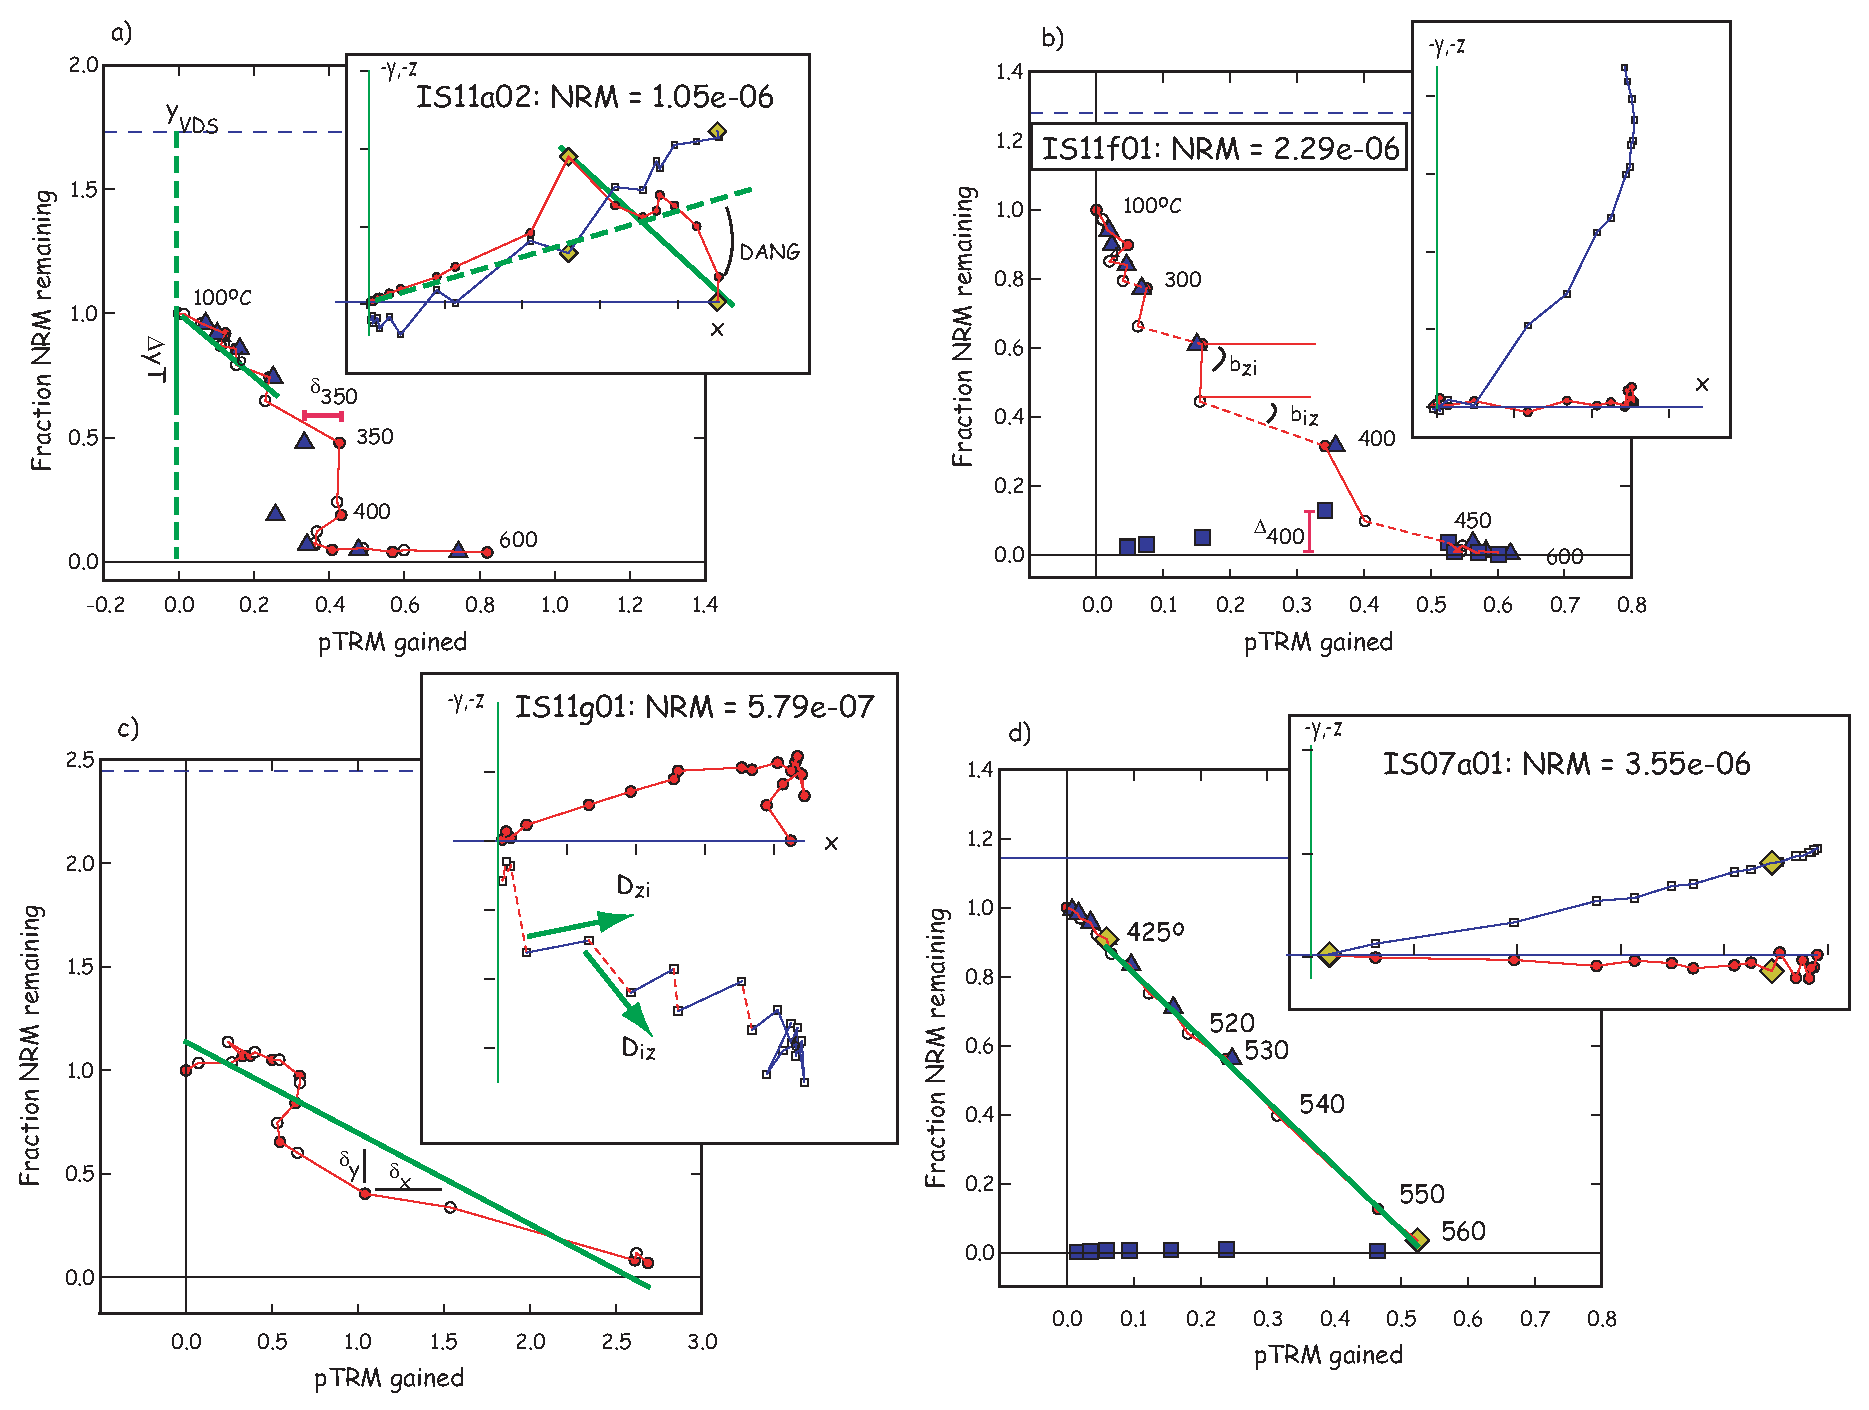
\includegraphics[width=14 cm]{EPSfiles/IZZI.eps}
\caption{Illustration of paleointensity parameters.  Arai plots:  The magnitude of the NRM remaining after each step is plotted versus the pTRM gained at each temperature step.  Closed symbols are zero-field first followed by in-field steps (ZI) while open symbols are in-field first followed by zero field (IZ).    Triangles are pTRM checks and squares are pTRM tail checks.     Horizontal dashed lines are the vector difference sum (VDS) of the NRM steps.   Vector endpoint plots:   Insets are the x,y (solid symbols) and x,z (open symbols) projections of the (unoriented) natural remanence (zero field steps) as it evolves from the initial state (plus signs) to the demagnetized state.   The laboratory field was applied along -Z.  Diamonds indicate bounding steps for calculations.   a)  The $f_{vds}$   is the fraction of the component used of the total VDS.  The difference between the pTRM check and the original measurement at each step is $\delta T_i$.      The inset shows the deviation angle (DANG) that a component of NRM makes with the origin.   The maximum angle of deviation MAD is calculated from the scatter of the points about the best-fit line (solid green line).  b) Data exhibit �zig-zag behavior� diagnostic for significant difference between blocking and unblocking temperatures.  The Zig-zag for slopes compares slopes calculated between ZI  and IZ steps ($b_{zi}$) with those connecting IZ and ZI steps $b_{iz}$).  The difference between the pTRM tail check and the original measurement at each step is $\Delta T_i$.   c) $\beta$ reflects the scatter  ($\delta_x, \delta_y$) about the best-fit slope (solid green line).  The Zig-zag for directions compares those calculated between ZI  and IZ steps ($D_{zi}$) with those connecting IZ and ZI steps $D_{iz}$).   [Figures from Ben-Yosef et al., 2008.]
}
\label{fig:IZZI}
\end{figure}
\nocite{benyosef08}


\begin{enumerate}
\item The Deviation of the ANGle (DANG; Tauxe and Staudigel, 2004; see Chapter 9):  The angle that the  direction of the NRM component used in the slope calculations  calculated as a best-fit line (see Appendix~\ref{app:eigen}) makes with the angle of the line anchoring  the center of mass (see Appendix~\ref{app:eigen}) to the origin (see insert to Fig.~\ref{fig:IZZI}a). 
\nocite{tauxe04}

\item The Maximum Angle of Deviation (MAD; Kirschvink, 1980; see Chapter 9):   The scatter about the best-fit line through the NRM steps.  \nocite{kirschvink80}

\item We can calculate the best-fit slope ($b$)  for the  data on the NRM-pTRM plot   and its standard error $\sigma$ (York, 1966; Coe et al. 1978).   \nocite{york66,coe78}
The procedure for calculating the best-fit slope, which is  the best
estimate for the paleofield, is  given as follows:

\begin{quote}
a)Take the $N$ data points that span two temperature steps $T_1$ and $T_2$, 
the best-fit slope $b$ relating the NRM ($y_i$) and the pTRM ($x_i$)
data in a least squares sense (taking into account variations in both
$x$ and $y$  is given by:

\begin{equation}
b=- \sqrt{ {\sum_i (y_i-\bar y)^2}\over {\sum_i (x_i-\bar x)^2} },
\label{eq:slope}
\end{equation}

\noindent where $\bar y$ is the average of all $y$ values and $\bar x$ is the
average of all $x$ values. 

b) The y-intercept ($y_o$) is given by $\bar y - b\bar x$.  

c) The standard error of the slope $\sigma$ is:

\begin{equation}
\sigma_b = \sqrt {
{2\sum_i (y_i -\bar y)^2 - 2b \sum_i (x_i-\bar x)(y_i-\bar y)}
\over
{(N-2)\sum_i(x_i-\bar x)^2}
}.
\label{eq:stderr}
\end{equation}
\end{quote}


\item The ``scatter'' parameter $\beta$:  the standard error of the slope $\sigma$ (assuming uncertainty in both the pTRM and NRM data) over  the absolute value of the best-fit slope $|b|$ (Coe et al. 1978).   


\item The remanence  fraction, $f$, was defined by Coe et al. (1978) as:

$$ f = \Delta y_T/ y_o,
$$
\noindent where $\Delta y_T$  is the length of the  NRM segment used in the slope calculation (see Figure~\ref{fig:IZZI}).    



\item The fraction of the total remanence  (by vector difference sum), $f_{vds}$ (Tauxe and Staudigel, 2004):  While $f  $ works well with single component magnetizations as in Fig.~\ref{fig:IZZI}d where it reflects the fraction of the total NRM used in the slope calculation, it can be misleading when there are multiple components  of remanence as in Fig.~\ref{fig:IZZI}a.   The values of  $f $ for such  specimens can be  quite high, whereas the fraction of the total NRM is much less.  We prefer to use a parameter $f_{vds}$ which is the fraction of the total NRM, estimated by the vector difference sum (VDS; Chapter 9) of the entire zero field demagnetization data.  The VDS (see Fig.~\ref{fig:IZZI}a)  ``straightens out'' the various components of the NRM by summing up the vector differences at each demagnetization step.   $f_{vds}$  is calculated as:

$$ f_{vds} = \Delta y_T/ y_{vds},$$

\noindent where $y_{vds}$  is the vector difference sum of the entire NRM  (see Figure~\ref{fig:IZZI}a and Chapter 9).      This parameter becomes small, if the remanence is multi-component, whereas the original $f$ can be blind to multi-component remanences. 





\item The Difference RATio Sum, DRATS:  The difference between the original pTRM at a given temperature step (horizontal component of the circles in Fig.~\ref{fig:IZZI}) and the pTRM check (horizontal component of the triangles in see Fig.~\ref{fig:IZZI}), $\delta_i$ (see Fig.~\ref{fig:IZZI}a), can result from experimental noise or from alteration during the experiment. Selkin and Tauxe (2000) normalized  the maximum $\delta_i$ value within the region of interest by the length of the hypotenuse of the NRM/pTRM data used in the slope calculation.  DRAT is therefore the  maximum difference ratio expressed as a percentage.  In many cases, it is useful to consider the trend of the pTRM checks as well as their maximum deviations.    We follow Tauxe and Staudigel  (2004) who used  the sum of these differences.  We normalize this difference sum by the pTRM acquired by cooling from the maximum temperature step used in the slope calculation to room temperature.  This parameter is called the Difference RATio Sum or DRATS.   Only pTRM checks at temperatures below the maximum bound are included in the DRATS calculation.

\item Maximum Difference \% MD\%:    The absolute value of the difference between the original NRM measured at a given temperature step (vertical component of the circles in Fig.~\ref{fig:IZZI}) and the second zero field step (known as the pTRM tail check) results from some of the pTRM imparted in the laboratory at $T_i$ having unblocking temperatures that are greater than $T_i$.   These differences ($\Delta_i$; see Fig.~\ref{fig:IZZI}b) are plotted as squares.  The Maximum Difference, normalized by the VDS  of the NRM and expressed as a percentage is the parameter  MD\%.  

\item Zig-Zag $Z$:   In certain specimens, the IZZI protocol leads to rather interesting behavior, described in detail by  Yu et al. (2004).   The solid symbols in Fig.~\ref{fig:IZZI} are the  zerofield-infield (ZI) steps  and the intervening steps are the infield-zerofield (IZ) steps (open circles).  Alternating the  two  results in a ``zigzag'' in some specimens.  
The zigzag can be in either the 
\index{diagrams!Arai}
Arai diagrams (compare slope of solid versus dashed line segments in Fig.~\ref{fig:IZZI}b)  or in the orthogonal projections or the zero field vectors  (compare directions of solid and dashed line segments in Fig.~\ref{fig:IZZI} c).   We therefore can define a parameter  $Z$ by testing the difference in either the two sets of slopes  or the two sets of directions between the IZ steps and the  ZI steps.     

To test the significance of the difference between the zero-field IZ directions and those from the ZI zero-field steps, we calculate F-test $(F_w)$ for Watson's test for common mean (Watson, 1983).  The zigzag for directions $Z_{dir}$ is  ratio $F_w/F_{(\nu,)}$  where $F_{(\nu)}$ is the critical value for $F$ at $\nu=2N-2$ degrees of freedom (at the 95\% level of confidence).   

 For the slopes, we calculate the mean  and variance of the  slopes for the IZ segments ($\bar b_{iz},\sigma_{iz}^2$)  and the ZI segments ($\bar b_{zi},\sigma_{zi}^2$).   The parameter $t_b$ is the $t$ test for the two means.
   The zigzag for the slopes $Z_{slope}$ is the ratio $t_b/t_{(\nu)}$ where $t_{(\nu)}$ is critical value for  $t$ with $\nu= N_{iz}+N_{zi}-2$ degrees of freedom (from a statistics table).  

If the difference between the sets of directions and slopes is less than 2$^{\circ}$ or both $Z_{slope}$ and $Z_{dir}$ are less than unity, then $Z=0$.  Otherwise $Z$ is the larger of $Z_{dir}$ and $Z_{slope}$.  

\item  The ``gap factor'' $g$ (Coe et al. 1978) penalizes  uneven distribution of data points and is:
$$
g= 1 - \bar \Delta \bar y/\Delta y_T,
$$

\noindent where  $\bar \Delta \bar y $ is given by :

$$
{\bar \Delta \bar y = } { 1\over {\Delta y_T}  } \sum_{i=1}^{i=N-1} \Delta y_i^2,
$$
\noindent and is the weighted mean of he gaps $\Delta y_i$ between the $N$ data points along the selected segment. 

\item The  Coe quality index $q$ combines the standard error of the slope, the NRM fraction and the gap factors by:

$$
q = \beta  f g .
$$

\noindent
   As data spacing becomes less uniform, $g$ decreases.  


\item   A quick and dirty test for the possibility of anisotropy of TRM is to compare the direction of the pTRM acquired in the laboratory field with the direction of the applied field.  The angle between these two at the maximum pTRM temperature used in the slope calculation  is defined here as $\gamma$.  If this exceeds more than a few degrees,  it is advisable to perform some sort of test for TRM (or ARM) anisotropy.   


\end{enumerate}

%\customlink{Anisotropy_in_paleomagnetism}
\chapter{Anisotropy in paleomagnetism}
\label{app:anis}
\setcounter{figure}{1}
\section{The 15 measurement protocol}
\label{app:K15}

The Jelinek (1978) \nocite{jelinek78}  15 measurement scheme is  illustrated in Figure~\ref{fig:meas15}.  This is the 
procedure recommended in the manual  distributed
with the popular Kappabridge susceptiblity instruments.  
In the 15
measurement  case shown in Figure~\ref{fig:meas15}, the design matrix is:

\begin{equation}
\A=
\pmatrix{
.5&.5&0&-1&0&0\cr
.5&.5&0&1&0&0\cr
1&0&0&0&0&0\cr
.5&.5&0&-1&0&0\cr
.5&.5&0&1&0&0\cr
0&.5&.5&0&-1&0\cr
0&.5&.5&0&1&0\cr
0&1&0&0&0&0\cr
0&.5&.5&0&-1&0\cr
0&.5&.5&0&1&0\cr
.5&0&.5&0&0&-1\cr
.5&0&.5&0&0&1\cr
0&0&1&0&0&0\cr
.5&0&.5&0&0&-1\cr
.5&0&.5&0&0&1\cr},
\label{eq:ajel}
\end{equation}

\noindent and
$\B={1\over {20}}\cross$
\begin{equation}
\pmatrix{
3&3&8&3&3&-2&-2&-2&-2&-2&3&3&-2&3&3\cr
3&3&-2&3&3&3&3&8&3&3&-2&-2&-2&-2&-2\cr
-2&-2&-2&-2&-2&3&3&-2&3&3&3&3&8&3&3\cr
-5&5&0&-5&5&0&0&0&0&0&0&0&0&0&0\cr
0&0&0&0&0&-5&5&0&-5&5&0&0&0&0&0\cr
0&0&0&0&0&0&0&0&0&0&-5&5&0&-5&5\cr}.
\label{eq:bjel}
\end{equation}


\begin{figure} [htb]
%\epsfxsize 12cm
%\centering \epsffile{EPSfiles/meas15.epsf}
\centering  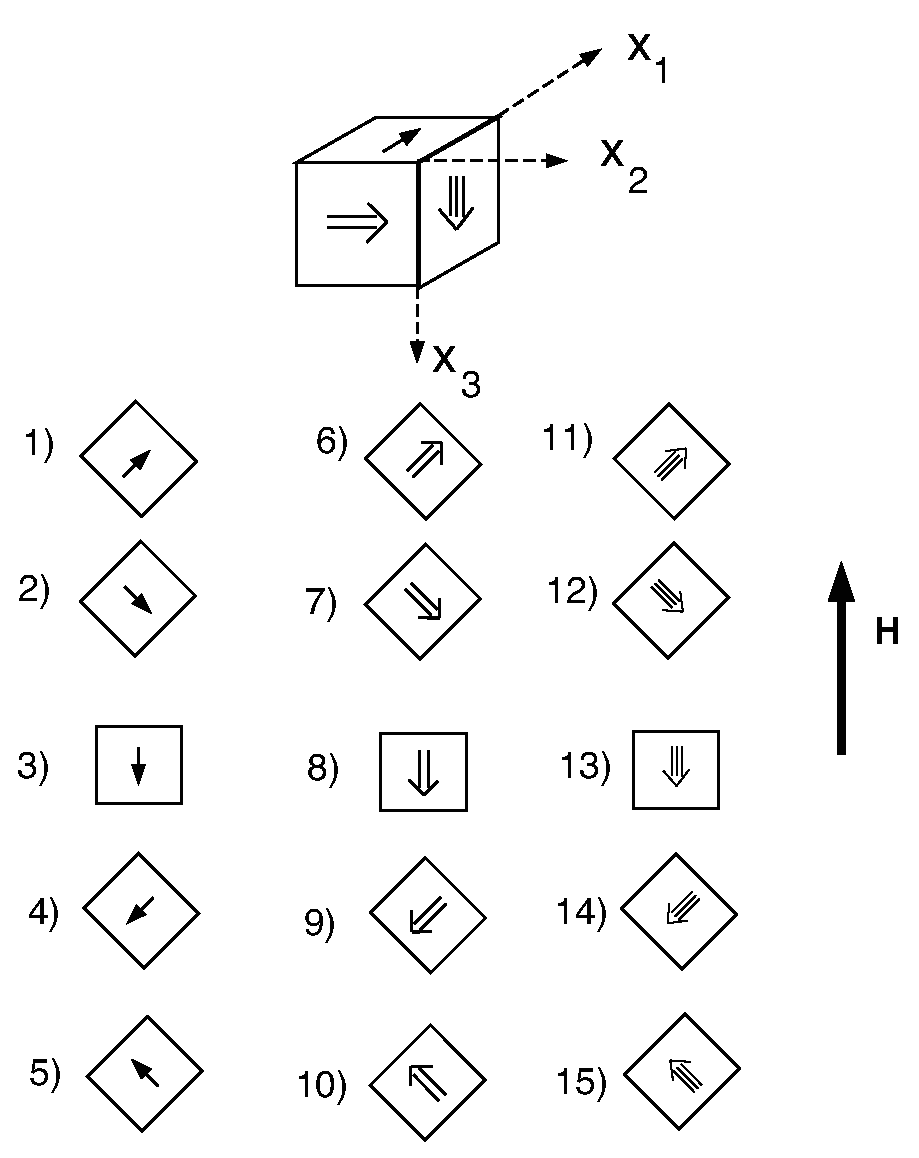
\includegraphics[width=12 cm]{EPSfiles/meas15.eps}
\caption
{ The 15  position scheme  of  
\index{Jelinek, V.}%
Jelinek (1976) for measuring the AMS of a
sample.  [Figure from Tauxe, 1998.] }
\label {fig:meas15}
\end{figure}

\clearpage

\section{The spinning protocol}
\label{app:AMSspin}


\begin{figure}[htb]

%\epsfxsize 10cm
%\centering \epsffile{EPSfiles/AMSspin.eps}
\centering  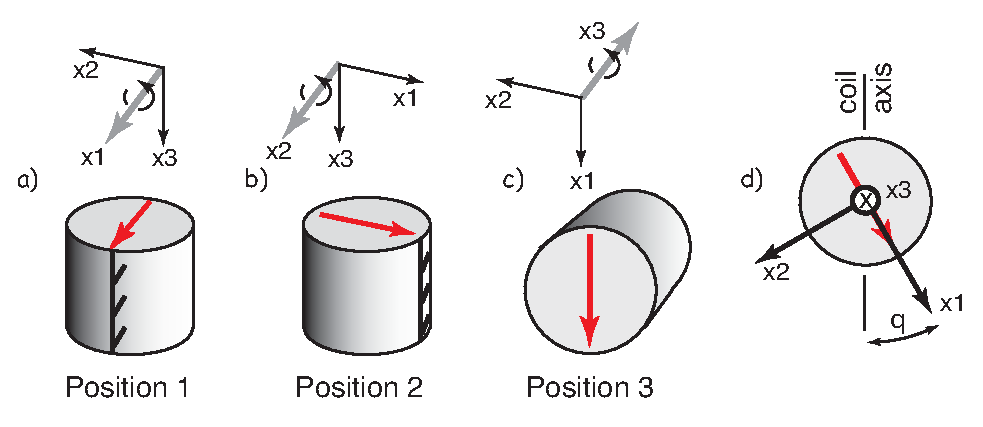
\includegraphics[width=10cm]{EPSfiles/AMSspin.eps}
\caption{Specimen orientations for the three spins used with spinning magnetic susceptibility meters. The heavy gray arrows
 show the axes of rotation; one oriented toward the user for Position 1 (a)  and 2 (b) away from the user for Position 3 (c). The
orientation of the specimen coordinate system in space is specified by the azimuth and plunge of either the arrow
along the core length (+x$_3$ axis, black) or the +x$_1$ axis (red arrow on core top). d) orientation of
applied field (coil axis) relative to specimen coordinates in Position 3. [Figure from Gee et al. 2008.]}
\label{fig:AMSspin}
\end{figure}
 \nocite{gee08}

\nocite{pokorny04}
More recent models of the Kappabridge magnetic susceptibility instruments (e.g., KLY-3S and KLY-4S; see e.g., Pokorny et al., 2004) measure anisotropy by spinning the specimen around three axes (Figure~\ref{fig:AMSspin}).     For complete measurement and analysis details, see Gee et al. (2008). \nocite{gee08} Here we just give the bare bones explanation. 

 The specimen is lowered into the measurement region and the susceptibility meter is set to zero.  The deviatoric susceptibility is then  measured in 64 positions per revolution for multiple  (often eight) revolutions (see Figure~\ref{fig:AMSspinProc}a.)    These data must corrected for instrumental drift (red line in the figure), adjusted to have zero mean and stacked (Figure~\ref{fig:AMSspinProc}b.)  The data can be fit with a best fit theoretical curve (red line in the figure).  The theoretical curve can be derived from the complicated design matrix (see Gee et al., 2008 for details).  As one example,  the measurement recorded at an angle $\theta_i$  (as shown in Figure~\ref{fig:AMSspin}d)  while spinning in Position 1 (Figure~\ref{fig:AMSspin}a)  is given by:

$$ 
K^{x1}_i = \chi_{22} \sin^2 \theta_i + 2\chi_{23} \cos \theta_i \sin \theta_i + \chi_{33} \cos^2 \theta_i.
$$

The best fit values for $\chi$ for the entire sequence of data gives the 2D Model for the set of data (see Figure~\ref{fig:AMSspinProc}b).   There are three such models for the measurement protocol, each yielding estimates of two of the three on-axis $\chi$ values ($\chi_{11}, \chi_{22}, \chi_{33}$).    These measurements are all adjusted to  zero mean susceptibility so one more measurement is required to determine the bulk susceptibility (the absolute susceptibility measured in the position shown in Figure ~\ref{fig:AMSspin}c or $\chi_{11}$ in Position 3.)      The three 2D models plus the bulk measurement are combined as shown in Figure~\ref{fig:AMSspinProc}d whereby the $\chi_{11}$ position in the 2D model for Position 3 is adjusted to the bulk measurement, and the best-fit 3D model is found that minimizes cross over errors for pairs of $\chi_{11}, \chi_{22}, \chi_{33}$.      Once the best fit values for $\chi$ are found and standard deviation, the data can be treated as described in Chapter 13.  

\begin{figure}[htb]
%\epsfxsize 14cm
%\centering \epsffile{EPSfiles/AMSspinProc.eps}
\centering  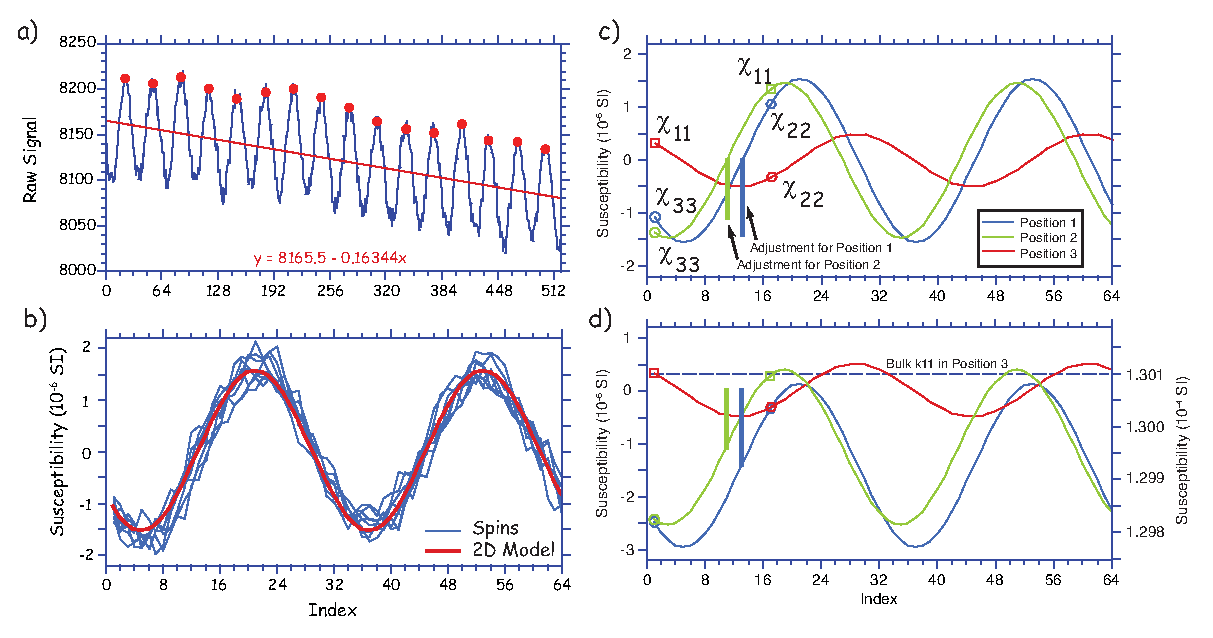
\includegraphics[width=14 cm]{EPSfiles/AMSspinProc.eps}
\caption{Processing steps for data spin protocol.  a) From a single spin with eight revolutions.  Raw data with peaks (red dots)
identified by peak-finding algorithm and best fit linear trend. Data are detrended using peaks. b) Data from detrended individual revolutions  and best fit 2-D model. c)  Original (zero-mean) deviatoric susceptibility data
from three spins. The best fit 2-D model for each spin provides an estimate of two elements of the deviatoric
susceptibility tensor (square, $\chi_{11}$; hexagon, $\chi_{22}$; circle, $\chi_{33}$). Thick bars indicate the calculated offsets for Positions 1 and 2. d) Crossover adjustment for data from three positions.  Original (zero-mean) deviatoric susceptibility data from three positions are scaled to absolute values (right-hand scale) using a bulk measurement in spin Position 3, and adjusted to minimize cross over error.    [Figure modified from Gee et al. 2008.]}
\label{fig:AMSspinProc}
\end{figure}


\section{Correction of inclination error with AARM}
\label{app:aarm}

\index{inclination!error!correction of}
The magnitude of ARM is here denoted $M_a$.
The  particle anisotropy is denoted  $a$ and  is given by:

\begin{equation}
a = \bigl[ {{M_{a_{||}} }\over {  M_{a_{\perp} } }}\bigr]_{particle},
\label{eq:a}
\end{equation}

\noindent where $M_{a_{||}}$ and $M_{a_{\perp}}$  are the magnitudes of the ARM acquired parallel to and perpendicular to the detrital particle long axis respectively.  
The normalized eigenvalues of the ARM tensor ($q_i$)  
 are defined as:
$$
q_i = { {M_{a_i}} \over {M_a} }.  
$$
\noindent Stephenson et al. (1986) defined an orientation distribution function for the preferred alignment of particle long axes whose eigenvalues are given by $\kappa_i$ where $\kappa_1 > \kappa_2 > \kappa_3$ as usual.   Jackson et al. (1991) collect together the two sources of anisotropy (alignment of particle long axes and individual particle anisotropies) as:

\begin{equation}
\kappa_i = {   {q_i(a+2) -1 } \over { (a-1) } }.  
\label{eq:kappa}
\end{equation}

Assuming that the DRM anisotropy is identical to the orientation distribution function of particle long axes we can combine and rearrange Equations~\ref{eq:flattening} and ~\ref{eq:kappa} to get the  relationship between the flattening factor $f$ and the ARM anisotropy:

$$
f= {{ q_3 (a+2)-1} \over { q_1 (a+2) -1} }  .
$$

From the foergoing, measuring the AARM tensor yields the values for $q$, but determining  values for $a$ are more problematic.      Vaughn et al.  (2005) describe a technique whereby magnetic particles are separated from the matrix, then allowed to dry in an epoxy matrix  in the presence of a magnetic field sufficient to fully align the long axes of the magnetic particles (say 50 mT).   The AARM parallel to and perpendicular to the axis of alignment therefore gives $a$ by Equation~\ref{eq:a}.  




\nocite{butler92}\nocite{scheidegger65}\nocite{fisher87} \nocite{tauxe04}
\nocite{york66} \nocite{coe78} \nocite{tauxe04}\nocite{selkin00}  \nocite{yu04} \nocite{watson83}\nocite{kirschvink80} \nocite{kirschvink80} \nocite{mcfadden82} 
\nocite{fisher87}\nocite{fisher87}\nocite{mcfadden88}\nocite{abramowitz70}
 \nocite{kent82}\nocite{mardia77} \nocite{tanaka99} \nocite{onstott80} 
\nocite{jelinek81}\nocite{tauxe90} \nocite{owens74} \nocite{nagata61} \nocite{balsley60} \nocite{stacey60} \nocite{woodcock77} \nocite{tauxe98} \nocite{vaughn05}\nocite{clement84} \nocite{clement04}\nocite{prevot93}  \nocite{clement91b}   \nocite{prevot93}\nocite{tauxe07} \nocite{masters00} \nocite{mcelhinny96b}\nocite{strik03}  \nocite{opdyke96} \nocite{kent99b}\nocite{constable03}
\nocite{berggren95} \nocite{gradstein95}
 \nocite{merrill96}\nocite{hatakeyama02}\nocite{johnson08}   \nocite{tauxe03b}
 \nocite{tauxe07}\nocite{prevot90} \nocite{mcelhinny97}\nocite{cox69}\nocite{constable88} \nocite{tauxe08} \nocite{tauxe04d,tauxe08}  \nocite{selkin00}
 \nocite{mcelhinny97} \nocite{tauxe04d} 
\nocite{tauxe08} 
\nocite{riisager05} \nocite{vandamme91,vandamme92}\cite{riisager02} \cite{plenier02} \nocite{stephenson86}



